\documentclass{jot}

\usepackage[utf8]{inputenc}
\usepackage[T1]{fontenc}
\usepackage[english]{babel}
\usepackage{microtype} % optional, for aesthetics
\usepackage{tabularx} % nice to have
\usepackage{booktabs} % necessary for style
\usepackage{multirow}
\usepackage{hyperref}
\usepackage{hypcap}
\usepackage{comment}

% \usepackage{graphicx}
\graphicspath{{./figs/}}
% \usepackage{listings}
% \lstset{...}

% \newcommand\code[1]{\texttt{#1}}
% \let\file\code


%%% Article metadata
\title{The Reaction of Open-Source Projects to New Language Features: \\
An Empirical Study of C\# Generics}
\runningtitle{An Empirical Study of Language Features}

\author[affiliation=ncsu, photo=donghoon, nowrap]
    {Donghoon Kim}
    {   is a PhD student in the Department of Computer Science at North Carolina State University, USA.
    His research is at the intersection of Software Engineering and Programming Languages. Previous, he had worked at Samsung Electronics, Korea (Republic of) after receiving his Master of Science Degree at Auburn University, USA.
        Contact him at \email{dkim2@ncsu.edu}, or visit \url{http://www4.ncsu.edu/~dkim2/}.}

\author[affiliation=ncsu,  photo=emerson, nowrap]
    {Emerson Murphy-Hill}
    {   is an assistant professor in the Department of Computer Science at North Carolina State University. His research interests include human-computer interaction and software tools. He holds a Ph.D. in Computer Science from Portland State University. Contact him at \email{emerson@csc.ncsu.edu}, or visit \url{http://www.csc.ncsu.edu/faculty/emerson}.}
        
\author[affiliation=gatech, photo=parnin, nowrap]
    {Chris Parnin}
    {   is a PhD student at the
Georgia Institute of Technology. His research
interests includes psychology of programming
and empirical software engineering. Contact him
at \email{chris.parnin@gatech.edu}, or visit \url{http://cc.gatech.edu/~vector}.}
    
       

\author[affiliation=msr, photo=bird, nowrap]
    {Christian Bird} 
    {is a researcher in the empirical software engineering group at Microsoft Research. He
is primarily interested in the relationship between software design, social dynamics, and processes in
large development projects. 
%EMH cuts this down a bit, to be congruent size-wise with others' bios
%He has studied software development teams at Microsoft, IBM, and in
%the Open Source realm, examining the effects of distributed development, ownership policies, and
%the ways in which teams complete software tasks. 
%He has published in the top software engineering
%venues and is the recipient of the ACM SIGSOFT distinguished paper award. 
Christian received his
Ph.D. from U.C. Davis under Prem Devanbu and was a National Merit Scholar at BYU, where he
received his B.S. in computer science. Contact him
at \email{cbird@microsoft.com}, or visit \url{http://www.cabird.com/}.}
 
\author[affiliation=ubc, photo=ronald, nowrap]
    {Ronald Garcia}
    {is an assistant professor in the Department of Computer Science at University of British Columbia, Canada. His research interests include programming language semantics, design, and implementation, including language support for library-centric and modular software development, generic and generative programming, and domain specific languages and libraries. Contact him at \email{rxg@cs.ubc.ca}, or visit \url{http://www.cs.ubc.ca/~rxg/}. }    
    

\affiliation{ncsu}{North Carolina State University, Raleigh, USA\\ \url{http://www.csc.ncsu.edu/}}
\affiliation{gatech}{Georgia Institute of Technology, Atlanta, USA\\ \url{http://www.cc.gatech.edu/}}
\affiliation{msr}{Microsoft Research, Redmond, USA \\ \url{http://research.microsoft.com/en-us/}}
\affiliation{ubc}{University of British Columbia, Vancouver, Canada \\ \url{https://www.cs.ubc.ca/}}
\runningauthor{Donghoon Kim et al.}

\jotdetails{
    volume=V,
    number=N,
    articleno=M,
    year=2012,
    doisuffix=jot.201Y.VV.N.aN
}


\begin{document}

\begin{abstract}

Language designers introduce new language features in programming languages 
because those features are claimed to be beneficial.
%New programming language features are motivated with speculative claims that problems
In this paper, we investigate claims made about the generics language feature,
and compare how those claims stack up in C\# versus Java.
% Although many languages offer the same functionality for a given feature, 
% they implement the feature in different ways.     
Through an empirical study of the generics feature in open-source projects, we found that  
(1) although they have the same claimed benefits in different programming languages, 
%generics are used more widely in C\# than in Java and that
generics are more readily used in C\# than in Java and that
the benefits of generics are manifested more clearly in C\# programs,
% Chris Parnin:
% push-back on this finding.  Is it not the case that this preference is contextual.
% Programmers certainly care about succinctness when things are too long.
% When things are more neutral, programmers take the side of readability:
%%and (2) software developers appear to prefer programming readability 
%%rather than succinct syntax when using generics. 
% How about this instead:
%[JOT_review]
and (2) programmers rarely use the \texttt{var} keyword with generics, except when using very long generic expressions,
suggesting that programmers prefer readability over succinct syntax, as long as the syntax does not become overly verbose.  
%(2) programmers are not likely to sacrifice program readability unless syntax becomes overly verbose.
% Chris Parnin:
% What we say is implementation will probably mean something else to a programming language person.
% I think we mean ecosystem, or user experience.
%%These results call for re-thinking the implementation of new language 
%%features beyond the claimed benefits of those features.
 
%[JOT_review] no change
Many of these observed differences may be attributed to subtle differences in implementation 
and are consistent with the notion that crafting the user experience of a programming language feature 
can impact how the feature is adopted and embraced by developers. 

\end{abstract}

\keywords{empirical study, generics, C\#, static analysis}

\section{Introduction}
Joanne is a hypothetical programming language designer at Goosoft. 
Her group has developed a special programming language 
used for smart phone applications. 
Two years after the language is released to the public, 
Joanne proposes to introduce a new feature to 
her programming language, a feature that she claims will
make programs more concise and reduce errors.
Similar language features have been
introduced in other programming languages.
In those languages, the feature has been designed 
in different ways and have had varying degrees of success. 
Thus, Joanne faces a problem;
how can she design her language feature to increase its probability of success?
What can she learn from past language features that can help improve future ones?
What \emph{do} we know about how developers use language features, anyway?
This paper is a step towards helping Joanne, and language designers like her,
answer such questions.

Joanne's story is an example of how
programming language designers evolve existing programming languages. 
They do this is by incorporating new language features that could potentially
resolve existing difficulties,
reduce programming effort, 
and increase developers' productivity.

%Such features are integrated with programming languages for the purpose of improving programming languages  \cite{Stroustrup:2007:ELR:1238844.1238848}. 
%aim to improve programming languages \cite{Stroustrup:2007:ELR:1238844.1238848}.
%Differences Between C++ Templates and C# Generics (C# Programming Guide) 
%http://msdn.microsoft.com/en-us/library/c6cyy67b.aspx

One such language feature is \textbf{generics}. 
%which Stroustrup \cite{Stroustrup:2007:ELR:1238844.1238848} considers to be  
%one of the most significant contributions to the software development community.    
%The generics feature 
%which are designed to support programming languages to be improved. 
As we outline in Section~\ref{section:related_work},
experts claim that generics have three main benefits:
it supports software reusability, 
it helps developers find errors earlier,
and it avoids the need for explicit type casting~\cite{DBLP:conf/oopsla/BrachaOSW98}.
%and (3) it supports syntactic convenience. 
%Because of these benefits, 
%the generics feature is implemented and supported differently within each language 
These claimed benefits have led language designers to integrate generics into 
several different programming languages~\cite{what_is_generics}.
%[FSE_review]
After Clu and Ada introduced the generics feature in the 1970's and 1980's respectively~\cite{Liskov_clu,ada_generics}, 
other programming languages such as C++, Java, and C\# incorporated generics as well.
Consequently, one might expect that developers would embrace generics
and reap all the benefits that generics have to offer.

%EMH to CP: this doesn't make sense to me -- trying again above
%the claimed benefits would extend to developers,
%as well as observed by wide use and less problems.

But to the programmer, all the academic quibbles on design 
implementation, 
and theory meld into a single 
user experience of using the new feature.
Programmers must not only contend with learning and 
applying the new feature but also deal with the 
complexities of backward capability, 
migration, and politics of using the feature in production code.
Can programmers really trust and realize all benefits 
claimed by researchers and language designers?  Will it be worth it? 

%Programming languages 
%New programming language features are created to resolve existing difficulties, reduce programming efforts, and increase development productivity.  
%In programming languages, 
%Software developers may demonstrate immediate effects of new programming language features when they use those features in a project.
%New programming language features may well show immediate effects when software developers use those features in a project. 
%For example,  
%the autoboxing feature eliminates the pain caused by the process of boxing 
%which requires a wrapper class (e.g. \texttt{Integer} in the case of \texttt{int}) since collections could only hold reference types.  
%as the generics feature is another example which has several benefits: 
%(1) it reduces code duplication by abstracting over types,
%(2) it moves run-time errors to compile-time errors by the generics type system, 
%and (3) it provides convenience by not using explicit casting operations. 
%Because of these benefits, the generics feature has been introduced in many programming languages such as C++, Java, and C\# 
%after the first adoption on Ada in the 1980s.

Research suggests that this expectation may not be realized for some 
languages such as Ada and Java. 
In Ada, Frankel~\cite{Frankel:1993:ERA:260096.260201} found that developers did not use generics as designed.
Although Ada generics were designed to allow developers to write reusable software, 
most developers did not use Ada generics for reusable software at all.
Instead, developers opted to create reusable software by other means.  
%since using Ada generics requires more efforts than       
%of the generics feature in Ada was different from the patterns Ada developers used   
%to accomplish 
%the benefits of \textquotedblleft reuse\textquotedblright \ in a software development project.
%Because the patterns for reusable software in Ada were indeed different from those previous defined, 
%many opportunities for reusable software did not require the use of Ada generics at all.
More recently, in a study of 40 open source Java projects, we showed that
generics in Java have been only narrowly used despite their many claimed benefits~\cite{java_generics_ese}.
%according to the experimental results of Java generics shown by Parnin \emph{et al.} \cite{java_generics_ese}.
%These results lead us to the challenge that how new language features are used in a project;
These results bring about questions concerning the broader usage of generics in practice.  
How are generics used in software projects written in other programming languages? 
Are they used in the same amounts and in the same ways, or different amounts and in different ways? 
What are the factors that influence the differences and similarities? 

       
We perform an empirical study of C\# generics 
to answer the above questions. 
For some parts of our study, we replicate our previous empirical study of 
generics in 20 established\footnote{In the previous paper~\cite{java_generics_ese}, we examined both \emph{recent} and
\emph{established} projects; the difference is that established projects were started before
generics were introduced into the language. In the present paper, we examine established
C\# projects, and compare our results to only the 20 established projects from 
the previous Java study.} 
Java projects~\cite{java_generics_ese},
and then compare the usage of generics between C\# and Java. 
We initially expected that the usage of generics in the two languages would be similar
because of the many similarities between C\# and Java.

%as the way Parnin \emph{et al.} did with Java generics \cite{java_generics_ese}. 
%and compare C\# generics with Java generics in this paper. 

%\noindent
%From these similarities and differences between the two languages, 
%we expect that the generics usage of the two languages may bring comparable results. 


We make the following contributions in this paper:
\begin{itemize}

	\item \textbf{Investigation of the claimed benefits of C\# generics}:
	%[FSE_review]
	we determine how the claimed benefits of C\# generics manifest in real open-source projects.   
	Our results suggest that generics help remove casts, 
	reduce duplication, and improve performance in real programs.
	 
	\item \textbf{Comparison of generics' use in C\# and Java}:
	we analyze open source Java and C\# projects to determine whether differences exist 
	in generics usage.
	As in Java, C\# developers appear not to migrate much existing code to use generics,
	but unlike Java, C\# generics are typically championed by more than one developer in a project.	
	
	\item \textbf{Exploration of the cause of different usage}:
	we explore some of the causes of the different usage of generics between C\# and Java.
	Our results suggest that implementation choice makes a difference in a language
	feature's success, and that developers appear to prefer readability over concision.  
	
	\item \textbf{Investigation of the interaction of generics and implicit typing}:
	we compare how often developers use generics in conjunction with C\#'s 
	\texttt{var} type.
	Our results suggest that developers typically do not use the two language features together, and
	instead typically declare generic types expicitly.		
	
\end{itemize}
  


The paper is organized as follows:
we introduce C\# generics in more detail in Section~\ref{section:background} 
and related work in Section~\ref{section:related_work};
%\section{Data Characterization}
we then formulate six research questions in Section~\ref{section:investigation}; 
we describe data characterization of 20 open source C\# projects in Section~\ref{section:data_characterization};
we investigate how C\# generics are used in those projects
and compare the results with our previous Java generics results in Section~\ref{section:investigating};
%We estimate how several benefits of generics are manifested.  
% We also analyze how C\# generics can improve performance based on the usage of value types, and 
% how implicit generic type declarations 
% %(\texttt{var} type) 
% are used.
%in Section \ref{section:distinctive_characteristics}.
and finally, we discuss why the usage of C\# generics is different from that of 
Java generics in Section~\ref{section:discussion}. 


\section{Background}
\label{section:background}

In this section, we compare C\# with Java to explain why we selected C\# for this study. 
We then explain generic terminology.
We also describe how generics are used in C\#, and explain
how C\# generics differs from Java generics.
%Finally, we define some special terminology we wil use to explain the results of our study.   
%because C\# generics have unique characteristics due to different generics implementation when generics are instantiated.
%Then, we define our terminology used in this paper.
%For example, C\# generics should be instantiated such as depending on instantiation from generics type declarations compared with Java generics nevertheless a syntactic syntax. Then, we define terminologies used in this paper.
%We cate\ell\diamondgorize to analyze the usage of generics as follows \ref{section:background}

\subsection{Comparison between C\# and Java}

In this paper, we selected the C\# programming language to compare with Java generics
because the two languages have several similarities, but also important differences.

C\# and Java are similar from a developer's point of view,
so a meaningful comparison between the two is possible.
Both C\# and Java are class-based, object-oriented languages
with garbage-collected runtimes and
both have \texttt{Object} at the top of their inheritance
and subtyping hierarchies.
Both languages base their design of generics around
f-bounded polymorphism~\cite{Canning:1989:FPO:99370.99392}.
Both languages have very similar syntax; 
the syntax at the statement and expression level is almost identical, 
but there are some minor differences in how generic classes and interfaces are declared.
%For example, on inheritance, Java uses explicit keyword such \texttt{extends} for classes and \texttt{implements} for interfaces 
%while C\# uses \texttt{:} (colon) for both classes and interfaces. 
%since C\# can infer this from the kind of types classes or interface derive from. 
%http://en.wikipedia.org/wiki/Comparison_of_C_Sharp_and_Java   
%Specifically, the two languages show a superficial syntactic similarity to generics.
Both languages introduced generics around the same time: 
Java in 2004 as part of J2SE 5.0 
and C\# in 2005 as part of .NET 2.0.

Like Java, C\# is widely used. 
According to the TIOBE Programming Community Index \cite{TIOBE:online}, 
an indicator of the popularity of programming languages, as of February 2012, 
Java is about twice as popular as C\#.
However, TIOBE remarks that C\# is arguably the only serious candidate to compete with Java
because the popularity of C\# is growing 
whereas the popularity of Java is decreasing.

C\# and Java take different approaches to the design of 
generics.
%http://download.oracle.com/javase/tutorial/java/generics/erasure.html  
Java generics are designed to allow for backward compatibility,
so that Java byte code generated from source code that uses 
generics can work with older versions of Java that do not have generics support.
In contrast, C\# generics do not allow for backward compatibility.
Another difference is that in C\# generics are designed specially
to improve performance when value types are used as generic arguments
so that these value types do not have to be converted into objects~\cite{DBLP:conf/pldi/KennedyS01}.
In contrast, Java has no such special case for value types
and requires that value types are converted into and from objects
when using generics,
incurring additional runtime overhead.
These design differences may make a substantial difference
in how developers use generics.

\subsection{General Terminology in Generics}
\label{subsection:general_terms}
% when to use generics collections http://msdn.microsoft.com/en-us/library/ms172181(v=VS.80).aspx
% generics terminology http://msdn.microsoft.com/en-us/library/ms172192.aspx#generics_terminology
C\# developers can define and use a generic class as in the following example: \\
\vspace{-10pt}
\begin{verbatim}
  1  public class MyStack<T>{ 			
  2	     T[ ] store;  		
  3      public void Push(T x){ ... }
  4      public T Pop(){ ... } 
  5      public void MyMethod<X>(X x){ ... }
  6  }
  7  MyStack<int> intStack = new MyStack<int>();
\end{verbatim}

\normalsize
\noindent 
Throughout this paper, we use the following terms:
\begin{itemize}
  
	\item A \textbf{generic type}: a class or interface declared with one or more type parameters using angle brackets. 
	%Angle brackets are the placeholder of any type. 
	An example is \texttt{MyStack<T>} on line \# 1.
	
	\item A \textbf{generic method}: a method declared with one or more type parameters using angle brackets. 
	An example is \texttt{MyMethod<T>} on line \# 5.
	
	\item A \textbf{generic type parameter}: a type variable defined in angle brackets.
	An example is \texttt{T} in \texttt{MyStack<T>} on line \# 1.
	
	\item A \textbf{generic type argument}: a type that substitutes for a generic type parameter.
	An example is \texttt{int} of \texttt{MyStack<int>} on line \# 7. 
	The \texttt{int} substitutes for \texttt{T} in \texttt{MyStack<T>} on line \# 1. 
	
	%\item A \textbf{generic type declaration}: a generic type that is declared by generic type parameters in a program. 
	%The above example program between line \#1 and \#11 is the complete of generic type declaration of \texttt{MyStack<T>}.
	
	\item A \textbf{parameterized type}: an instantiation of a generic type with generic type arguments.
	%[Ron_Review]
	MyStack<int> is an example of a parameterized type on line \# 7. 
	 
\end{itemize}

%The definition of a \textbf{generic type} is a class or interface that has 
%such as \texttt{class} and \texttt{interface} is defined by 
%angle brackets, 
%which are the placeholders of \textbf{generic type parameters} (e.g. \texttt{Dictionary<TKey, TValue>}). 
%Every type can substitute for 
%each generic type parameter, 
%which we call a \textbf{generic type argument}. % substitutes for with any type called a \textbf{generic type argument}.
%For example,
%the \texttt{Dictionary<int, string>} is the  
%generic type which has two generic type arguments, \texttt{int} and \texttt{string}.  
%can substitute for \texttt{Dictionary<TKey, TValue>}.
%A \textbf{generic type argument} is any type that is substituted for a generic type parameter. 
%, which enclose a generic type parameter in C\#, Java, and C++.
%A generic type declared by generics type parameters is called a \textbf{generic type declaration}.
%A \textbf{parameterized type} is an instantiation of a generic type declaration with generic type arguments.
%A \textbf{raw type} is an instantiation of a generic type declaration without generic type arguments. 
%The following is the examples of an instantiation in C\# code: \\

%\texttt{//parameterized type} 

%\texttt{Queue<int> numbers = new Queue<int>();} \\

%\texttt{//raw type}

%\texttt{Queue numbers = new Queue();} \\
%font size
%\tiny
%\scriptsize
%\footnotesize
%\small
%\normalsize
%\large
%\Large
%\LARGE
%\huge
%\Huge

\subsection{Generic Uses in C\#}
\label{subsection:generics_csharp}

In this paper part of our analysis is concerned with both how people declare generic types
and how people use generic types.
In this section, we describe the various ways generic
types can be used.

%[JOT_review] a little modified...
A common example of where generics are useful is in declaring
variables that are collections.
Before C\# generics, \texttt{System.Collection}
was the default namespace from which collections were imported.
%[JOT_review] added ``2005 as part of .NET 2.0,'' to help a reviewer understand
When generics were introduced in 2005 as part of .NET 2.0, 
in a design decision aimed at encouraging adoption of generics,
the default collection namespace became \texttt{System.Collections.Generic}.
This new namespace included a whole new set of generic collections.  
Many types in the old collection namespace, such as \texttt{ArrayList}, 
did not have any corresponding generic types in the new namespace.  
Instead, new generic collections, such as \texttt{List<T>} were introduced.  
This decision effectively made developers have to explicitly include the old namespace 
if they wanted to continue to use the older \texttt{ArrayList}, 
to override the default choice of a \texttt{List<T>}.  
Further, this might have made migration easier as there was no name 
collision between the generic and non-generic collection namespaces.
However, some types, such as the \texttt{Queue} class, belong to both the 
\texttt{System.Collection} and the \texttt{System.Collections.Generic}  
namespaces.

In our previous paper~\cite{java_generics_ese}, we investigated how often
generic types in Java were used as a \emph{raw type}.
%[Ron_Review]
A raw type is a generic type that is used without type arguments~\cite{igarashi2001recipe}.
For instance, if \texttt{MyStack<T>} were written in Java, a programmer could
use it in a raw way like so: \texttt{MyStack s;}.
In Java, a generic type can be used as either a parameterized
type or as a raw type.
Using raw types is more succinct than using generics, but the programmer sacrifices the compile-time
type safety checks that come with generics.

In this paper, we are interested in how often raw types are used in C\#,
but C\# generics can only be used as parameterized types. 
%[JOT_review] added this to help a reviewer understand... 
This is an important implementation difference between C\# generics and Java generics.  
%[Ron_Review]
A ``raw type'' in this study means a collection
%[Ron_Review] 
that is used from \texttt{System.Collection} for which
there is an equivalent type in \texttt{System.Collections.Generic}.
Examples of such collections include \texttt{Queue}, 
and \texttt{SortedList}.%, and \texttt{Stack}.


%%%%%%%%%%%%%%%%%%%%%%%%%%%%%%%%%%%%%%%%%%%%%%
%%%%%%%%%%%%%%%%%%%%%%%%%%%%%%%%%%%%%%%%%%%%%%
%%%%%%%%%%%%%%%%%%%%%%%%%%%%%%%%%%%%%%%%%%%%%%
\section{Related Work}
\label{section:related_work}

%In this section, we discuss previous claims about, implementation and studies of generics.

%\subsection{Claims Regarding Generics}

%There are several references which show the pros and cons of the generics feature  
%among different programming languages
%because different programming languages take different approaches to implement the generics feature due to their characteristics.
%%
%%
%%
%Skeet \cite{csharp_in_depth} asserts that
%C\# generics are better than Java generics in almost every respect
%while Java generics have some nice features:
%(1) Java retains backwards comparability for generics.
%(2) Java developers do not need to learn new classes which can be used with Java generics.
%(3) Java supports generic variance using wildcards.
%%
%%
%%
%Pryor \cite{jonathan_comparision2} compares Java generics and C\# generics,
%and especially addresses how generics implementation has an important influence on 
%what generics code can do and what can be done at run-time as follows:
%(1) Java and C\# generics look very similar in their syntax,
%(2) Their compiler assists checking types related to generics,
%and (3) C\# generics have additional performance benefits due to allowing value types, removing the overhead of boxing.
%%
%%
%%
%Garcia \emph{et al} \cite{Garcia03} show a comprehensive comparison of generics in several languages
%and evaluate them as follows:
%\begin{itemize}
%  \item In C++, templates are just a means for compile-time polymorphism 
%  (compile-time binding between abstract type and concrete type).
%  There is no performance loss at run-time.
%  Excessive use of templates may lead to significant increases in executable size.
%  \item Java generics provide enough support for generic programming to allow a type-safe implementation,
%  but there are several problems 
%  (e.g. subtyping-constrained polymorphism, and unnecessarily duplicate code for declaring and initializing a variable) 
%  that make writing generics tiresome and restricted. 
%  For example, 
%  \item C\# generics overcome some of the inconvenience of Java generics;
%  value types are allowed to be arguments for generic type parameters.
%\end{itemize}


%The purpose of our research is to analyze the usage of C\# generics based on the claims 
%that the generics feature has several benefits.
Several prior researchers and practitioners have claimed that generics are beneficial.
%Due to the benefits of generic programming, many programming languages adopt the generics feature.
%The benefits of the generics feature are manifested in a project.
In C++, Austern~\cite{C++generics} claimed that using templates can 
prevent code duplication by allowing a class with different data types.
In Java,
Bracha \cite{bracha04} claimed that they considered type-safety as a primary design goal of generics.   
Garcia \cite{Garcia03} claimed that Java generics provide a type-safe design.
Bloch \cite{Effective_Java} claimed that generics  
support finding errors at compile-time, not at run-time
and eliminate typecasts.
% and expressive benefits of generics
%generics do not need to do a type cast manually and find errors at compile-time, not at run-time.
%so using multiple data types at each template can prevent code duplication.
In C\#, 
Lowy \cite{intro_CSharp_generics} claimed
generics let developers reuse code, and 
Skeet \cite{csharp_in_depth} claimed that generics have benefits such as compile-time type safety and performance improvements.
Several researchers have claimed that C\# generics improve performance 
\cite{Garcia03,jonathan_comparision2,intro_CSharp_generics,DBLP:conf/pldi/KennedyS01}.
Based on these claims, we formulated research questions 
to analyze how such claimed benefits are manifested in practice. 
 
Some existing papers have shown empirically that some of these benefits 
are manifested in several languages. 
Basit \emph{et al.} \cite{DBLP:conf/seke/BasitRJ05} showed that 
the generics feature prevents code duplication in practice with class libraries in C++ and Java. 
In this paper, we extend this result to C\#.
Laurentiu \emph{et al.} \cite{DBLP:conf/synasc/DraganW05} showed 
the performance results of generics using a benchmark that they implemented, 
where they compared generics and specialized code 
in several programming languages (e.g. C++, Java, C\#, and Aldor).
They found that using generics is not as efficient as specialized code.  
In contrast, in this paper we estimate performance improvements 
based on generics in real open source projects, rather than a benchmark.
This builds on our previous work where we investigated how the generics 
feature is used in Java projects~\cite{java_generics_ese}.
 
%based on the performance overhead of each generic type between value types and reference types. 
%and then estimate performance improvement in real applications such as open source projects, not a benchmark. 
% how the generics feature affects performance gain in a project.     

%EMH doesn't think this is relevant enough
% Other research has investigated empirically other languages.
% Calla{\'u} \emph{et al.} \cite{DBLP:conf/msr/CallauRTR11} investigated 
% how the dynamic and reflective features of programming languages are used in the Smalltalk language. 
% They assessed how much these features are actually used and  
% what kinds of projects used more those featuers in the top 1,000 projects based on the size.  

As we mentioned in the introduction, 
Frankel~\cite{Frankel:1993:ERA:260096.260201} 
found that generics were not widely used in Ada.
Later, the principal designer of Ada suggested that, if he could,
he would eliminate parameterized types, because they were 
``less useful than originally thought''~\cite{Ryder:2005:ISE:1101815.1101818}.
%[FSE_review]
In this paper, we empirically investigate the usage of generics in a number
of dimensions for the C\# language.


\section{Study Approach}
\label{section:investigation}

In this section, we explain the approach in this study. 
Section \ref{subsection:comparison} introduces our research questions.
%Section \ref{subsection:benefits_generics_feature} related to the benefits of the generics feature, 
%and 
%Section \ref{subsection:distinctive_characteristics} related to the distinct characteristics of C\# generics.
Section \ref{section:projects_studied} introduces the characteristics of 20 projects collected for this study. 
Section \ref{section:methodology} introduces the framework and the procedures we used
for analyzing those projects.  
  

\subsection{Research Questions}
\label{subsection:comparison}

\newcommand{\idea}[3]{
\vspace{1mm}
\begin{quote}
\textbf{#1} (\textbf{#2}) - #3
\end{quote}
\vspace{1mm}
}

\newcommand{\hypothesis}[2]{\idea{Hypothesis #1}{H#1}{#2}}
\newcommand{\researchQ}[2]{\idea{Research Question #1}{RQ#1}{#2}}

%[FSE_review]
In this section, we describe 6 research questions,
of which 
four are from the research questions we used in our Java 
generics study\footnote{We reformatted two hypotheses in the previous paper~\cite{java_generics_ese}
into research questions in the present paper, because several readers found the mix of
research questions and hypotheses confusing.}
and two new research questions are introduced to analyze specific characteristics of C\# generics.     

%Thus, we replicated an empirical study of Java generics that Parnin \emph{et al.} conducted \cite{java_generics_ese}, 
%we use the hypotheses and research questions used by Parnin \emph{et al.} \cite{java_generics_ese},  
%and then compared Java generics with C\# generics. \\  

As we mentioned in related work, experts claim that 
generics reduce the need for typecasting,
which in turn reduces runtime errors~\cite{Effective_Java,DBLP:conf/oopsla/BrachaOSW98,csharp_in_depth}.
%EMH does the C# compiler really insert casts?
%Answer: No,  
%No, Reflection can be used to create new realizations for new combinations of type parameters.
%http://en.wikipedia.org/wiki/Comparison_of_C_Sharp_and_Java%This is because, with generics, the compiler inserts correct casts implicitly.
%
%
%The compiler compares the type of the local variable on the left of an assignment statement 
%to the return type of the code on the right of an assignment statement generated by implicit type casting of generic type arguments at compile-time. 
While we would like to determine directly whether runtime errors are really
reduced in open source projects, we found very few bug reports
where InvalidCastExceptions are reported.\footnote{For example, see 
\texttt{http://bugzilla.xamarin.com/buglist.cgi?quicksearch=InvalidCastException}}
We suspect that this is because developers find and fix 
InvalidCastExceptions before releasing their software.
Instead of measuring whether runtime errors are actually reduced when
generics are used, we measure whether type casts are 
reduced:

%[FSE_review]
\researchQ{1}{Will the number of type casts in a codebase be reduced when generics are introduced?}


%A compiler compares the type of the local variable on the left of an assignment statement 
%to the return type of the code on the right of an assignment statement generated by implicit type casting of generic type arguments at compile-time.
%Because implicit type casts replaces explicit type casts, using generics reduces the number of type casts.
%For example,
%List\textless string\textgreater list = new List\textless string\textgreater ();\\
%\indent list.add("abc"); \\
%\indent int i = list.get(0); // compile-time error
%Queue<int> genericQueue = new Queue<int>();
%			rawQueue.Enqueue(1);
%			rawQueue.Enqueue("s");
%			
%			int i2 = (int)rawQueue.Dequeue();
%			i2 = (int) rawQueue.Dequeue();
%Parnin \emph{et al.} \cite{java_generics_ese} indicates that \textbf{Java generics do not support Hypothesis 1}.
%The primary motivation for using generics is to move run-time errors to compile-time errors
%because a compiler detects a return type of the code generated by implicitly casting of generic type parameters at compile-time.
%Such implicit casting replaces an explicit type cast. Thus, using generics reduces the number of type casts.
%Nevertheless, Parnin \emph{et al.} \cite{java_generics_ese} showed that \textbf{their empirical results of Java generics do not support Hypothesis 1}.
%
%
%%%%%%%%%%%%%%%%%%%%%%%%%%%%
%Our empirical results of C\# generics seem unlikely to support Hypothesis 1, 
%because C\# generics also have such the same claimed benefit that generics reduce the number of run-time errors.  \\
%because some generic collections in C\# such as \texttt{ArrayList} and \texttt{Hashtable} in \textbf{r-only} still should be used as a raw type regardless of the introduction of generics.  
%because not all collections in C\# can be used as a parameterized type
%(72.5\%) 
%due to \textbf{r-only},  
%while every collections in Java can be used as a parameterized type. \\
% (100\%).  \\
%%%%%%%%%%%%%%%%%%%%%%%%%%%
\noindent
In our previous study
%\footnote{We are in the process of correcting the digital library version of paper where it was incorrectly reported as not supporting the hypothesis.} 
our empirical results showed that generics reduce casts in Java (RQ1)~\cite{java_generics_ese}.
%~\footnote{The authors changed the conclusion of H1 with newly analysis.} }.
%Our empirical results of C\# generics seem to support Hypothesis 1 
%since the programming pattern using generics is similar between C\# and Java. \\  
%because not all collections in C\# can be used as a parameterized type
%while every collections in Java can be used as a parameterized type. \\
We expect similar results in C\# in this study.

Other experts have claimed that generics reduce 
duplication~\cite{C++generics} because
generics reduce the need to redefine similar classes.
For example, supposed we used our \texttt{MyStack} class from 
Section~\ref{subsection:general_terms} as follows:

\begin{verbatim}
  MyStack<int> intStack = new MyStack<int>();  
  MyStack<string> strStack = new MyStack<string>();
\end{verbatim}

\noindent
Without generics, a developer would normally create two stack classes, such as: 

\begin{verbatim}
  class IntMyStack{
      public void Push(int x){ ... }
      public int Pop(){ ... }
  }
  class StringMyStack{
      public void Push(string x){ ... }
      public string Pop(){ ... }
  }
\end{verbatim}

\noindent
Thus, each developer-defined generic class can prevent the code duplication, but
only if it is parameterized with more than one argument.
We formulate this research question as:

%below program format : http://files.slembcke.net/misc/JavaGenericSpecialization.pdf
%[FSE_review]
\researchQ{2}{Does the introduction of developer-defined generic types reduce code duplication?}

\noindent
Our previous study with Java shows that generics can prevent code 
duplication (RQ2) \cite{java_generics_ese},
and we expect similar results with C\# in this study.


%Another motivation for using generics is to reduce code duplication
%because generics permit common parameterized types such as \textless S, T\textgreater \ which will be replaced by specific types such as \textless int, int\textgreater \ or \textless double, double\textgreater
%when generics are instantiated.
%By reducing code duplication with generics, a program prevents general negative effects of duplicated codes such as code bloat and software maintenance (e.g. fixing copied bugs).

%\textbf{Java support Hypothesis 2} \cite{java_generics_ese}. We expect that C\# supports this because Hypothesis 2 is the general benefit of generics.   \\

Once a team decides to use a compiler that supports generics,
the team may make a collective decision to use generics,
or individuals may take the initiative on their own.
Thus:

\researchQ{3}{Will project members broadly use generics after introduction into the project?}

\noindent
Previously we observed that Java generics are usually 
introduced by one or two contributors who champion their 
use and that broad adoption by the project community is 
uncommon~\cite{java_generics_ese}.

Not only can software developers use generics in new code,
but they can also migrate old code that was developed before
generics.
Thus:

\researchQ{4}{Will there be large-scale efforts to 
convert old code using raw types to use generics?} 

\noindent
Previously we found that most Java projects did not show a 
large scale conversion of raw to parameterized 
types~\cite{java_generics_ese}.
In C\#, we expect that the rate of migration is lower
than in Java because some non-generic collections
in old namespace do not have 
generic counterparts in the new namespace.
%\texttt{System.Collections.Generic}.


%most of generic collections are added in C\# 2.0
%Most of generic collections 
%\textbf{p-only} 
%which
%are created in C\# 2.0. 
%Some of the non-generic collections such as \textbf{r-choice} can be used as a parameterized type such as \textbf{p-choice}.
%%%%%%%%%%%%%%%%%%%%%%%%%%
%%%%%%%%%%%%%%%%%%%%%%%%%%
%\noindent
%\textbf{Research question 3} (\textbf{RQ3}) - Does generics support in the IDE influence adoption? \\
%\indent
%Parnin \emph{et al.} \cite{java_generics_ese} showed that
%\textbf{lack of IDE support for generics did not have an impact on its adoption}.
%Java is independent of IDEs.
%Although Java integrated IDEs such as Eclipse, Netbeans, and IntelliJ IDEA support generics, 
%not all IDEs supported generics when they were first introduced.
%
%%Thus, generics support in the IDE may not influence adoption.
%
%On the other hand, C\# is closely dependent on IDEs such as Microsoft Visual Studio.
%C\# programs run on the .NET framework, an integral Windows component.
%For example, with the release of Visual Studio 2005, the C\# language has been updated to version 2.0.
%Visual Studios offers numerous features that make programming endeavors much simpler. 
%Accordingly, most C\# developers may prefer IDEs.
%However, as Troelsen \cite{IDE_exception} claims, 
%a small number of C\# developers might reject IDEs 
%%when they may want to access some functions of the underlying compiler, which IDEs alone do not support, such as the generation of multifile %assemblies.
%%that some C\# developers might reject IDEs 
%%when they may want to access some functions of the underlying compiler, which IDEs alone do not support.
%%For example, Visual Studio 2005 does not support the generation of multifile assemblies \cite{IDE_exception}.
%Thus, RQ3 is inappropriate for the C\# language because C\# language is closely dependent on IDEs,
%so we do not solve the RQ3 in this study.  
%
%Instead of RQ3, we trace when the first parameterized type appears in a project.
%Table \ref{table:20projects} shows the date when the first parameterized type is shown in a project.
%Although we have not found yet the information when C\# 2.0 (Visual Studio 2005) has been used at each project for using generics,
%The \emph{mono} project used generics even before generics were officially released 
%because the libraries of generics classes in C\# 2.0 were implemented and tested by the \emph{mono} and Microsoft .NET~\cite{c5_generic}.
%The \emph{lucene.net} project shows 1st P-type in June 2008, which is the very last.
%We note that the time gap between first and last P-type dates for 1st P-type among projects is around 3 years.
%This information may give a hint how long it takes to adopt new feature in a project. 
%In the future work, we plan to investigate what factors affect the decision of when to begin using generics.
%
%

%: 
%(1) the performance gain made by allowing value types that do not incur boxing and unboxing and 
%(2) the succinct declaration of generic types by the \texttt{var} type. \\  

Another claimed benefit of C\# generics is a performance improvement~\cite{intro_CSharp_generics}.
Without generics, if a value type is placed into a collection of objects,
that value type must be converted to an object (boxing) and 
converted from an object when removed from the collection (unboxing).
Such collections thus incur processing overhead when boxing and unboxing. 
However, C\# generics do not require boxing and unboxing for value types
because the actual values, not objects, are held in generic types that 
are parameterized with a value type.
Thus:

%[FSE_review]
\researchQ{5}{Does the use of C\# generics improve performance in a program?}
%\footnote{The performance means the run-time of the code using generics} 


%due to the additional processing overhead of boxing and unboxing operations.
% 
%Boxing is the process of converting a value type to the type \texttt{object} and unboxing is the process to extract the value type from the %\texttt{object}.
%Value types are stored directly on the stack so they can be accessed directly, such as \texttt{int}, \texttt{double}, and \texttt{char}.
%On the contrary, 
%reference types are stored on the run-time heap so they can be accessed through a reference to that storage, such as the \texttt{object} type.
%For example, collections can only hold the \texttt{object} so value types require boxing operation.      
%Generic collections in C\# do not incur the boxing and unboxing of value types. 
%(e.g. \texttt{int}, \texttt{string}, and \texttt{double}). 
\noindent
Previous work suggests that C\# generics do improve performance,
at least in benchmarks~\cite{DBLP:conf/pldi/KennedyS01}.
%have up to a 200\% performance gain by placing value types in a place of type arguments and a 100\% performance gain with reference types. 
%They also indicate that the application as a whole may or may not achieve improvements in performance \cite{intro_CSharp_generics}. 
%For example, \texttt{int} in their code is 4.5 times faster than \texttt{object}, and
%\texttt{double} in their code is 5 times faster than \texttt{object}.  
%\texttt{object}\---same, \texttt{int}\---4.5 times, and \texttt{double}\---5 times. 
However, it is currently unknown whether performance 
is improved in the wild because previous
work has not explored how often developers use value types with
generic collections in real C\# programs.
We initially expected that such use is common.

A language feature that was introduced after generics, yet may
work synergistically with them, is the \texttt{var} keyword,
which supports implicit typing of local variables.
Introduced in C\# 3.0 in November 2007, the \texttt{var} keyword
offers succinct syntax to declare generic types compared 
with explicitly typed generics. 
For example, using explicit typing, we would declare the following 
local variables like so:

\begin{verbatim}
  Dictionary<string,int> data 
  				         = new Dictionary<string,int>();
  List<List<int>> list 
                   = new List<List<int>>();             
\end{verbatim}
%//nested generics
\noindent
The \texttt{var} keyword can reduce the repetitive typing in these examples like so:

\begin{verbatim}
  var data = new Dictionary<string,int>();
  var list = new List<List<int>>();
\end{verbatim}

\normalsize
\noindent
There is no performance difference between explicit generic type declarations and implicit ones
%The \texttt{var} type has no run-time overhead 
because the \texttt{var} keyword instructs the compiler to 
infer the exact type from the right side of the initialization statement at compile-time.
Moreover, the IntelliSense feature, also known as auto-complete, in Visual Studio
is aware of the exact type of a var-typed local variable, 
and can assist the developer equally well in both implicitly and 
explicitly typed versions of the code.
This leads to our final research question:

%[FSE_review]
\researchQ{6}{Do C\# developers choose implicit 
generic type declarations more often than explicit ones?}

\noindent
However, it is not clear whether the benefits of the \texttt{var} keyword
are outweighed by the readability drawbacks~\cite{var_readability}.
Specifically, one might argue that readability is decreased because
the type represents a compiler-checkable specification that documents
the developer's intent; with the \texttt{var} keyword, that intent 
becomes obscured.
Indeed, this research question is a specific form of the more general question,
``are developers willing to write specifications?''
Our initial suspicion was that developers will generally prefer
to use the succinct syntax of the \texttt{var} keyword.


%The following C\# code shows that the \texttt{var} type hinders the readability of the code: \\
%Consider the following C\# code: \\
%\scriptsize
%\texttt{var tomorrow = DateTime.Today.AddDays(1);} \\
%\indent
%\texttt{DateTime tomorrow = DateTime.Today.AddDays(1);} \\
%\normalsize
%\noindent
%The second statement is more readable than the first statement
%because it provides the return type information. 
%
%
%while the return type of the second statement is the \texttt{DateTime} type, which clearly indicate .  


\subsection{Projects Studied}
\label{section:projects_studied}


%%%%%%%%%%%%%%%%%%%%%%%%%
%%%Table 20 projects
\begin{table}[ht!]
\small
\begin{center}

\begin{tabular}{llr}

\textbf{Project Name} & \textbf{Type} & \textbf{LOC} \\
   \hline
AnkhSVN (ankhsvn)	        & application & 85,736	\\
Banshee (banshee)	        & application & 130,440	\\
Beagle (beagle)	          &	application & 174,611	\\
Boo Programming Language (boo) & library	&	89,816	\\
Castle (Castle)	          &	library     & 235,487	\\
CruiseControl.NET (ccnet)	& application &	175,042	\\
Cuyahoga (cuyahoga)	      & library     & 27,894	\\
F-Spot (f-spot)	          &	application & 90,862	\\
Jayrock (jayrock)	        &	library     & 52,031	\\
Apache log4net (log4net)	&	library     & 45,979	\\
Lucene.Net (lucene.net)	  &	library     & 154,984	\\
MediaPortal (mediaportal)	&	library     & 592,214	\\
Mono (mono)	              & library     & 3,125,097	\\
MonoDevelop (monodevelop)	&	application & 164,710	\\
Gendarme (mono-tools)	    &	application & 71,168	\\
Worldwind C\# (nasa-exp)	&	library     & 417,803	\\
NHibernate (nhibernate)	  &	library     & 292,379	\\
%Scrolling Game Dev. Kit 2 (sgdk2) & library	&	81,889	\\
Smuxi-IRC Client (smuxi)	&	application & 39,532	\\
Tomboy (tomboy)	          &	application & 35,419	\\
Zedgraph (zedgraph)     	&	application &	21,520	\\
 
\end{tabular}
\end{center}
\vspace{-10pt}
\caption{The 20 C\# projects under investigation.}
\label{table:20projects}
\end{table}


%%%%%%%%%%%%%%%%%%%%%%%%%
%%%Table 20 projects
%\begin{table*}[h!]
%\scriptsize
%\begin{center}

%\begin{tabular*}{13.2cm}{@{\extracolsep{\fill}}p{4cm}rrrrrrr}

%\textbf{Project Name} &\textbf{Type}&\textbf{Devs}&\textbf{Start}&\textbf{End}&	\textbf{1st P-type} & \textbf{LOC} \\
%   \hline\\

%AnkhSVN(ankhsvn)	&	15		&	8	&	1/23/2003 	&	3/8/2011 	&	2/27/2008 		&	85,736	\\[1mm]
%Banshee(banshee)	&	43		&	6	&	6/20/2005 	&	3/14/2011 	&	7/2/2006 	&	130,440	\\[1mm]
%Beagle(beagle)	&	34		&	7	&	4/29/2004 	&	2/18/2011 	&	9/19/2007 		&	174,611	\\[1mm]
%Castle(Castle)	&	31		&	6	&	10/20/2004 	&	3/14/2011 	&	12/7/2005 	&	235,487	\\[1mm]
%CruiseControl.NET(ccnet)	&	37		&	8	&	4/22/2003 	&	3/4/2011 	&	8/16/2007 		&	175,042	\\[1mm]
%Cuyahoga(cuyahoga)	&	4	&	7	&	5/23/2004 	&	2/5/2010 	&	11/30/2007 		&	27,894	\\[1mm]
%F-Spot(f-spot)	&	37		&	7	&	11/8/2003 	&	2/20/2011 	&	4/10/2008 	&	90,862	\\[1mm]
%Jayrock(jayrock)	&	2		&	5	&	9/7/2005 	&	3/22/2011 &	10/26/2007 		&	52,031	\\[1mm]
%Apache log4net(log4net)	&	5		&	6	&	1/28/2004	&	10/13/2010 	&	none		&	45,979	\\[1mm]
%Lucene.Net(lucene.net)	&	7		&	5	&	11/21/2005 	&	4/5/2011 	&	6/25/2008 	&	154,984	\\[1mm]
%MediaPortal(mediaportal)	&	97		&	7	&	4/21/2004 	&	6/24/2011 	&	11/5/2005		&	592,214	\\[1mm]
%Mono(mono)	&	274		&	9	&	6/8/2001 	&	3/17/2011&	4/7/2004 		&	3,125,097	\\[1mm]
%MonoDevelop(monodevelop)	&	55		&	5	&	9/23/2005 	&	3/18/2011 	&	6/4/2006		&	164,710	\\[1mm]
%Gendarme(mono-tools)	&	34	&	8		&	4/23/2005 	&	3/17/2011 	&	10/26/2006 		&	71,168	\\[1mm]
%Worldwind C\#(nasa-exp)	&	25		&	5	&	10/5/2004 	&	9/6/2010 	&	9/2/2006		&	417,803	\\[1mm]
%NHibernate(nhibernate)	&	26		&	8	&	2/17/2003 &	3/16/2011 	&	1/2/2006 		&	292,379	\\[1mm]
%Scrolling Game Development Kit 2(sgdk2)	&	1	&	5	&	2/25/2006 	&	3/5/2011 	&	2/6/2008 		&	81,889	\\[5mm]
%Smuxi-IRC Client(smuxi)	&	6		&	6	&	5/28/2005 	&	6/26/2011 	&	4/17/2007 		&	39,532	\\[1mm]
%Tomboy(tomboy)	&	30		&	6	&	9/18/2004 	&	1/9/2011 	&	1/2/2007		&	35,419	\\[1mm]
%Zedgraph(zedgraph)	&	7	&	4	&	8/23/2004 	&	12/12/2008 	&	3/28/2006		&	21,520	\\[1mm]

%AnkhSVN(ankhsvn)	&	application	&	15		&	1/23/2003	&	3/8/2011	&	2/27/2008		&	85,736	\\[1mm]
%Banshee(banshee)	&	application	&	43		&	6/20/2005	&	3/14/2011	&	7/2/2006		&	130,440	\\[1mm]
%Beagle(beagle)	&	application	&	34		&	4/29/2004	&	2/18/2011	&	9/19/2007		&	174,611	\\[1mm]
%Castle(Castle)	&	library	&	31		&	10/20/2004	&	3/14/2011	&	12/7/2005		&	235,487	\\[1mm]
%CruiseControl.NET(ccnet)	&	application	&	37		&	4/22/2003	&	3/4/2011	&	8/16/2007		&	175,042	\\[1mm]
%Cuyahoga(cuyahoga)	&	library	&	4		&	5/23/2004	&	2/5/2010	&	11/30/2007		&	27,894	\\[1mm]
%F-Spot(f-spot)	&	application	&	37		&	11/8/2003	&	2/20/2011	&	4/10/2008		&	90,862	\\[1mm]
%Jayrock(jayrock)	&	library	&	2		&	9/7/2005	&	3/22/2011	&	10/26/2007		&	52,031	\\[1mm]
%Apache log4net(log4net)	&	library	&	5		&	1/28/2004	&	10/13/2010	&	none		&	45,979	\\[1mm]
%Lucene.Net(lucene.net)	&	library	&	7		&	11/21/2005	&	4/5/2011	&	6/25/2008		&	154,984	\\[1mm]
%MediaPortal(mediaportal)	&	library	&	97		&	4/21/2004	&	6/24/2011	&	11/5/2005		&	592,214	\\[1mm]
%Mono(mono)	&	library	&	274		&	6/8/2001	&	3/17/2011	&	4/7/2004		&	3,125,097	\\[1mm]
%MonoDevelop(monodevelop)	&	application	&	55		&	9/23/2005	&	3/18/2011	&	6/4/2006		&	164,710	\\[1mm]
%Gendarme(mono-tools)	&	application	&	34		&	4/23/2005	&	3/17/2011	&	10/26/2006		&	71,168	\\[1mm]
%Worldwind C\#(nasa-exp)	&	library	&	25		&	10/5/2004	&	9/6/2010	&	9/2/2006		&	417,803	\\[1mm]
%NHibernate(nhibernate)	&	library	&	26		&	2/17/2003	&	3/16/2011	&	1/2/2006		&	292,379	\\[1mm]
%Scrolling Game Dev. Kit 2(sgdk2)	&	library	&	1		&	2/25/2006	&	3/5/2011	&	2/6/2008		&	81,889	\\[5mm]
%Smuxi-IRC Client(smuxi)	&	application	&	6		&	5/28/2005	&	6/26/2011	&	4/17/2007		&	39,532	\\[1mm]
%Tomboy(tomboy)	&	application	&	30		&	9/18/2004	&	1/9/2011	&	1/2/2007		&	35,419	\\[1mm]
%Zedgraph(zedgraph)	&	application	&	7		&	8/23/2004	&	12/12/2008	&	3/28/2006		&	21,520	\\[1mm]

%\end{tabular*}
%\end{center}
%\vspace{-10pt}
%\caption{The 20 C\# projects under investigation}
%\label{table:20projects}
%\end{table*}

%Table~\ref{table:20projects} displays the characteristics of the 
%20 open source C\# projects we selected.
%The column headings are defined as follows:
%\begin{itemize}
%  \item \textbf{Project Name} is the official name of each project. 
%  We use a shorter name (in parentheses) to refer to each project in this paper. 
  %\item Name in DB - development project name used in source repository (root directory name) so we keep this name in our database server to analyze data and use them on tables and figures in this paper.
%  \item \textbf{Type} is whether the project is an \emph{application}, primarily intended for an end-user, or a library, primarily intended for a developer,
%  \item \textbf{Devs (Developers)} is the number of committers to a project.  
  %\item \textbf{Age} is how many years of the project's history.
  %\item Type(Y) - the total duration from start to end by revision information.
%  \item \textbf{Start} is the start date of a project based on its version history.
%  \item \textbf{End} is the date of the last commit that we analyzed.     
%  \item \textbf{1st P-type} is the date when the first parameterized type appeared in the project.
  %\item C\#(\%) - the percentage of C\# used in a project from ohloh.net
%  \item \textbf{LOC} is the number of lines of C\# code in the project as measured by ohloh.net on July 2011. 
%\end{itemize}


We analyzed 20 open source projects to examine the research questions we introduced in 
the previous section.
%While Parnin \emph{et al.} \cite{java_generics_ese} selected the top most used projects,
We selected C\# projects in the same way we selected projects for our previous study
in Java~\cite{java_generics_ese}, that is, we used 
Ohloh.net's listing of the ``most used'' open-source projects,
then chose projects based on several criteria: 

\begin{enumerate}
	\item Each project should have more than 10,000 lines of C\# code.
	\item Each project should begin before C\# 2.0 was released in November 2005 
	%[FSE_review]
			so that we can observe how existing C\# projects incorporate the new language feature. 
	\item Each project should have a complete version history because 
			we want to trace the history of the project from its start. 
\end{enumerate}

\noindent
%All projects that we selected meet all three criteria, except one project.
%[Ron_review]
%The exception is \emph{sgdk2}, which began shortly after generics were
%introduced into C\# and generics were actually introduced into that
%project well after the project used raw types. 
%We had a difficult time finding 20 projects which meet all three criteria 
%because most of C\# projects started after C\# 2.0 on investigation. 
%Accordingly, the \emph{sgdk2} project was selected as a credible alternative.

Table~\ref{table:20projects} displays the name of each project,
whether the project is an \emph{application}, primarily intended for an end-user, 
or a \emph{library}, primarily intended for a developer,
and how many lines of code and the number lines of
C\# code in the project as measured by ohloh.net on the 
date we copied the project for analysis.
A table providing more details about each project is provided
in the Appendix\footnote{\url{http://www4.ncsu.edu/~dkim2/research/csharp_generics_appendix.pdf}} of this paper.
Overall, regarding the 20 projects, we observe that:

\begin{itemize}
  \item The total number of lines of code in 20 C\# projects (6,022,724 lines) was much smaller 
  than that of 20 established Java projects (548,982,841 lines) that we analyzed previously~\cite{java_generics_ese}. 
  We speculate that our C\# projects were smaller than our Java projects both because
	the Java projects tended to be older and more mature. 
	%Because the size is different by about two orders of magnitude between C\# and Java projects, 
	%and maybe more widely used.  
  %The size of overall C\# projects is smaller than that of Java projects. 
 
  %\item The number of C\# developers and the lines of code vary.
  %There was no close relationship between developers and lines of code.
  
  %\item The average age was 6.7 years. Most projects have released their products.
  
  \item The first parameterized type in most of projects appeared 
  within one or two years of the official release of generics. 
  The \emph{mono} project was the first, introducing its first 
  parameterized type in April 2004,
  while the \emph{lucene.net} project was the last, introducing 
  its first parameterized type in June 2008. 
  
  \item The \emph{log4net} project never used parameterized types, because 
  although \emph{log4net} was built on several frameworks, including .NET Framework 2.0, 
  it appears that \emph{log4net} does not use many features, such as generics,
  which are not supported in .NET 1.0
  for backward compatibility~\cite{log4net:online}. 
  %DO : refer this link - http://logging.apache.org/log4net/release/framework-support.html
	\item That there did not appear to be a significant relationship between type of project and number of generics,
	by a two-tailed t-test.  That is, libraries did not appear to use generics more or less than applications.
\end{itemize}


Although we analyzed all of these projects, throughout this paper,
for the sake of brevity we focus our discussion on the top three projects 
based on the total number of parameterized types and raw types.
We discuss the other 17 projects when these three projects are not
adequately representative. 
The top three C\# projects are as follows:
\begin{itemize}
  \item \textbf{\emph{mono}} - An implementation of the C\# platform and .net designed to allow developers to easily create cross platform applications. 
  This is the largest project, 
  the oldest, and has the largest number of developers among the 20 projects. 
 % The number of raw types is higher than that of parameterized types. \\
  \item \textbf{\emph{nhibernate}} - An object-relational mapping framework for .NET software projects.
  It has the 2nd largest total number of parameterized types and raw types,
  although it is the 4th largest project and has 10th largest number of developers. 
  %\item \emph{monodevelop} - An IDE primarily designed for C\# and other .NET languages. This project is relatively young, over 5 years old. 
  %The increasing rate of parameterized types is much higher than that of raw types after generics introduced. \\
  \item \textbf{\emph{mediaportal}} - A media center application for 
  listening, recording, and organizing music, movies, radio, and TV. 
  It has the 3rd largest total number of parameterized types and raw types,
  is the 2nd largest project, and has the 2nd largest number of developers.   
\end{itemize}
%
%
%\begin{table}
%\vspace{-30pt}
%\centering
%\begin{tabular}{l p{9.0cm}}
%\textbf{\emph{mono}} : & A software platform designed to allow developers to easily create cross platform applications. 
%  This is the largest project, 
%  the oldest, and has the largest number of developers among the 20 projects. \\
%\textbf{\emph{nhibernate}} : & An object-relational mapping framework for .NET software projects.
%  It has the 2nd largest total number of parameterized types and raw types although it is the 4th largest project 
%  and has 10th largest number of developers. \\
%\textbf{\emph{mediaportal}} : & A media center application (e.g. listen, record, and organize music, movies, radio, and TV). 
%  It has the 3rd largest total number of parameterized types and raw types 
%  although it is the 2nd largest project and has the 2nd largest number of developers.  \\  
%\end{tabular}
%\label{tbl:steps}
%\vspace{-30pt}
%\end{table}

\subsection{Procedure}
\label{section:methodology}

We reused our existing Java program analysis framework, written in Java and Python \cite{java_generics_ese}. 
However, we modified the framework to enable it to analyze C\# code
by implementing a C\# program extractor that extracts the 
information we needed to answer our research questions,
such as the number of type casts, raw types, parameterized types, \texttt{var} type declarations.
In order to implement the C\# program extractor, 
we used \emph{NRefactory}, a parser library for C\#~\cite{nrefactory:online}.  
%Our data and tools will be available in the some repositories.
Our framework analyzes the code as follows:
download the full history of each project from a remote development
repository using Git or Subversion to a local machine;
check out every version of every file from a project's repository, 
store the different file revisions in an intermediate format,
and transfer this information to a database;
extract generics information from each file revision
and populate the database server with this information;
and finally analyze the data in the database in respect to each research question.


%%%%%%%%%%%%%%%%%%%%%%%%%%%%%%%%%%%%%%%%%%%%%%
%%%%%%%%%%%%%%%%%%%%%%%%%%%%%%%%%%%%%%%%%%%%%%
%%%%%%%%%%%%%%%%%%%%%%%%%%%%%%%%%%%%%%%%%%%%%%
\subsection{Data Characterization}
\label{section:data_characterization}


\subsubsection{Project Adoption}\label{subsection:projects}

%[FSE_review]
To get an overview of adoption of the generics feature in C\# projects,  
we investigate the usage of C\# generics in the 20 selected projects.  
%
We measured the number of both parameterized types 
and raw types to observe how generics are adopted.

\begin{figure}[!ht]
\centering
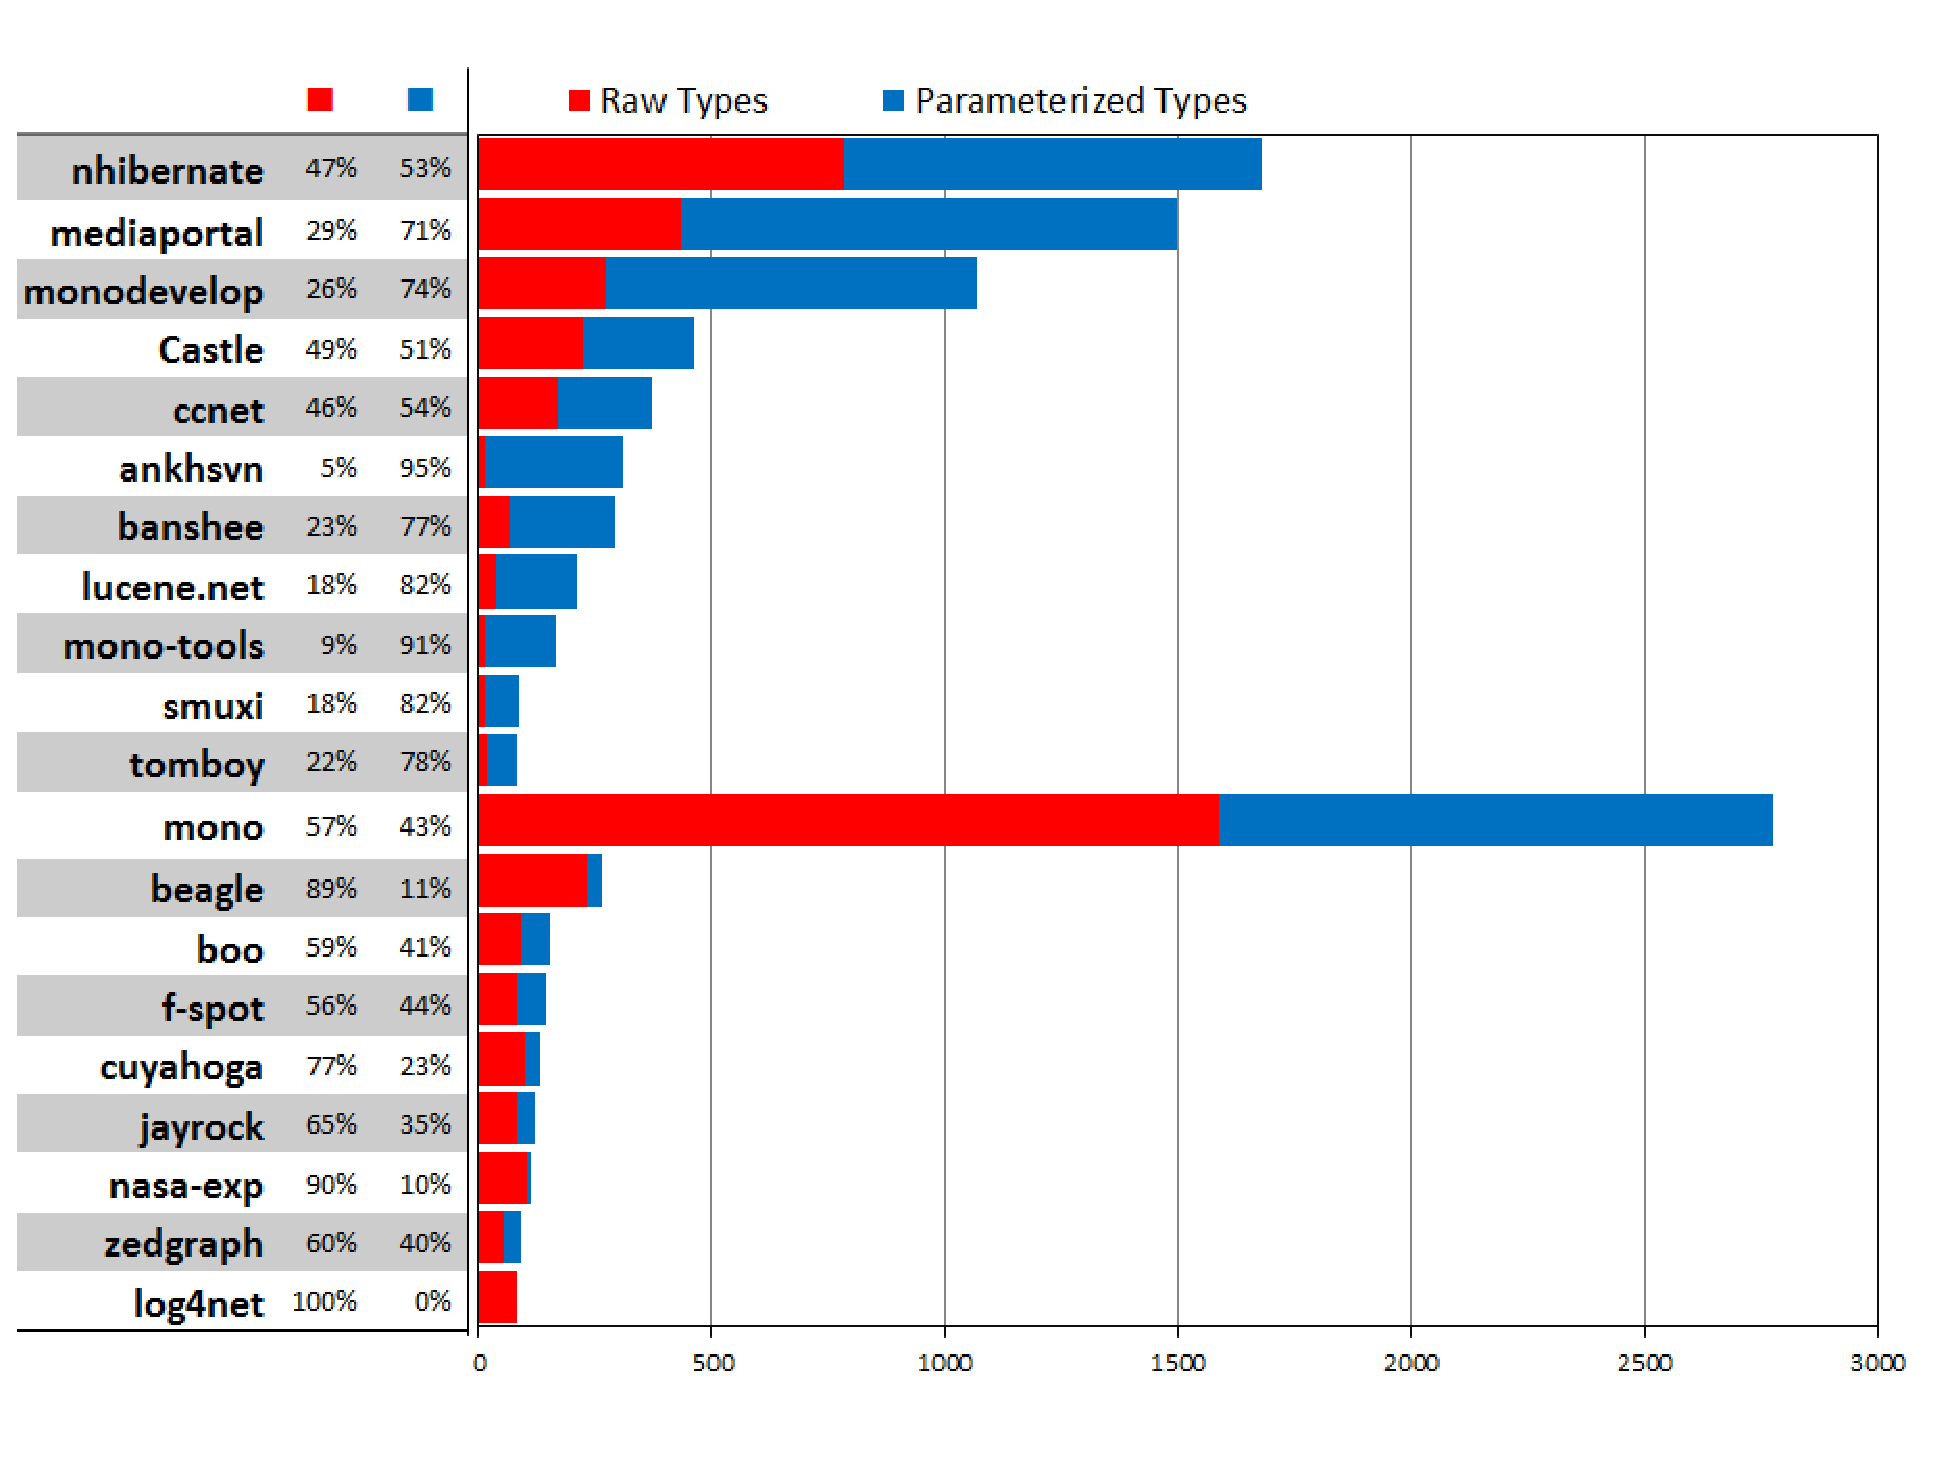
\includegraphics[width=0.8\textwidth]{figure1-0924-2013.eps}
\vspace{-12pt}
\caption{Total usage of raw and parameterized types. 
11 projects (above the \emph{mono} project) have more parameterized types (\textcolor{blue}{blue}, right) than raw types (\textcolor{red}{red}, left).}
\label{tab:total_raw_para}
\end{figure} 

%We characterize the collected data as a overview. 
%[JOT_review]
Figure \ref{tab:total_raw_para} shows the total usage of raw types and parameterized types with the percentage of each type---the ratio of raw types to parameterized types---in a project on the date of the last commit that we analyzed. 
%\textbf{X-axis represents 20 projects in order of predominant paramterized types projects by the total number and the Y-axis is the number.}
In C\# projects, 11 projects have more parameterized types than raw types 
while 8 projects used more raw types than parameterized types, 
and only one project, \emph{log4net}, did not use generics at all.
In Java projects~\cite{java_generics_ese},
8 out of 20 established projects used more parameterized types than raw types,
and 5 projects did not use generics at all.
%[FSE_review]
To determine whether the adoption rate of generics between the two groups (20 C\# projects and 20 Java projects) is different, 
we used the t-test to compare the ratio of raw types to parameterized types, 
using a two-tailed distribution assuming unequal variance. 
%[JOT_review] review this! => undid! (deleted)
From the result of the t-test ($p > .05$), we can conclude that there is no significant 
difference between the C\# projects' use of generics and that of Java projects. 
%However, we realized that know that this indicates that more C\# projects adopted generics than Java projects. 
%We note that the number of \emph{p-only} is larger than that of \emph{p-choice} among all nineteen projects.
%These results are different from Java generics Parnin \emph{et al.} conducted \cite{java_generics_ese} 
%in which 8 out of 20 projects used more parameterized types than raw types,
%and 5 projects did not use generics at all. 
In the 19 projects using generics, we found that by the latest point in development,
developers used more collections that existed solely in the \texttt{System.Collections.Generic}
namespace than collections that had implementations that existed in both \texttt{System.Collections}
and \texttt{System.Collections.Generic}. 
In other words, developers tended to use collections that 
\emph{only} had generic versions.



\begin{comment}
\subsubsection{Developer Adoption}\label{subsec:developers}
%count(distinct r.userID) parameterized :219
%count(distinct r.userID) rawtypes : 332
%count(distinct r.Revision) parameterized : 8782, boo:114, sgdk2: 7 ->8889 
%count(distinct r.Revision) raw types : 9527, boo:486, sgdk2: 91 ->9922
%count(distinct userID) total users : 638
%count(distinct r.userID) parameterized_declaration :153 (add 8 users to paramterized_types)
%total users : 638 + 8 = 646
%count(distinct r.Revision) parameterized_declaration_commit : 2673
We next investigated how many C\# developers use generics.   
We examined commits with creation or modification of both parameterized types, which include generic type declarations and generics method declarations, and raw types.  We term these commits ``associated'' with generics or raw types respectively.
%TOTAL : 770, duplicated ID : 132

% CAB - I don't think the text below is relevant to this paper
%Based on identifiers of those making commits in each project, 
%we found several developers (17.1\%) committed 
%to more than one project. 

%boo: Raw-4users, Parameterized-6users both:4
%boo: commit:2815, sgdk2:166
%boo: 
In total, 646 developers made 112,363 commits to the projects. 
Of those developers, 224 used generics (34.6\%),  
335 developers used raw types (51.8\%), 
and 187 developers used both generics and raw types (28.1\%).
For each developer, the average number of commits that introduced or modified 
parameterized types is 41 commits and 
the average associated with raw types is 30 commits.
The total number of commits associated with parameterized types is 8,889;
the total number associated with raw types is 9,922.
The data suggests that a smaller number of developers use
%(create or modify)
parameterized types more frequently 
than the larger number of developers use raw types.

%, by analyzing each developer who used parameterized types,
%whether most of the developers use generics widely or a few of the developers use generics more frequently to answer RQ1, 
%the generics usage by developers in Section \ref{subsection:generics_by_developers}. 
%We will use these results during the discussion about the adaption of generics in \ref{subsection:internal_structure}.
\end{comment}


\subsubsection{Common Parameterized Types and Arguments}
\label{subsection:feature_breakdown}

%\begin{table}[!ht]
%\begin{center}
%\includegraphics[width=3.4in]{types.eps}
%\label{figure:types}
%\end{center}
%\caption{Number of Parameterizations of different generics in nhibernate}
%\label{table:types}
%\end{table}

\begin{table}[!ht]
\small
\centering
 \begin{tabular}{lr}

\textbf{Type}		&	\textbf{Count}	\\
\hline
\texttt{ISet<string>}*	&	\texttt{55}	\\
\texttt{List<string>}*	&	\texttt{36}	\\
\texttt{List<int>}*	&	\texttt{21}	\\
\texttt{IList<Student>} &	\texttt{19}	\\
\texttt{IList<string>}	&	\texttt{17}	\\
\texttt{IDictionary<string,string>}&	\texttt{16}	\\
\texttt{ISet<T>}*	&	\texttt{15}	\\
\texttt{IDictionary<string,TypedValue>}	&	\texttt{15}	\\
\texttt{List<T>}*	&	\texttt{14}	\\
\texttt{IList<Person>}		&	\texttt{14}	\\
\texttt{IDictionary<string,Player>}	&	\texttt{14}	\\
\texttt{IList<Parent>}		&	\texttt{13}	\\
\texttt{List<Boolean>}*		&	\texttt{12}	\\
\texttt{List<Object>}*		&	\texttt{11}	\\
\texttt{List<TypedValue>}*	&	\texttt{10}	\\
\texttt{List<IType>}*	&	\texttt{10}	\\
\texttt{Dictionary<string,string>}*		&	\texttt{10}	\\
\texttt{IDictionary<TKey,TValue>}	&	\texttt{9}	\\
\texttt{IEnumerator<string>} &	\texttt{8}	\\
\texttt{IEnumerable<Column>}	&	\texttt{8}	\\
\end{tabular}

\vspace{-5pt}
  \caption{Number of parameterizations of different generics in \emph{nhibernate}.}
  \label{table:types}
\end{table}

We next analyzed which parameterized types were used and 
what the common arguments were to those types.
%which parameterized types and type arguments are used?
Table \ref{table:types} shows the top 20 parameterized types 
with distinct type arguments in the \emph{nhibernate} project. 
These 20 generic types cover about 43\% of generics in the project.
\texttt{ISet<String>} is the most used (23.1\%) combination, while     
\texttt{List} is the most commonly used (37.7\%) type.
%Overall, the \emph{List}-family such as \texttt{List} and \texttt{IList} is the most commonly used in this project (58.6\%).

As was the general trend in all projects,
in \emph{nhibernate} we found that the percentage of collections
used that were only available generically (64.2\%) 
is higher than that collections that are available
in both generic and non-generic versions (35.8\%).
An asterisk (*) next to a type name in Table~\ref{table:types}
denotes the collections that are only available generically.

While the usage of patterns of different generics 
vary from one project to the next, the 
\texttt{List}-family of types is the most used overall in 
the projects we studied.
%EMH not sure what the point of this is; these are just other types that projects used?
%such as \texttt{KeyValuePair}, \texttt{HashSet}, \texttt{Dictionary}, and \texttt{Nullable}.
Similarly, in open-source Java projects we found that 
\texttt{List}-family types were the most 
popular~\cite{java_generics_ese}.
   
% primitive type : http://msdn.microsoft.com/en-us/library/aa711900(VS.71).aspx
%Default Values Table (C# Reference) : http://msdn.microsoft.com/en-us/library/83fhsxwc.aspx

We also investigated which type arguments were used.
% Type arguments are closely related to generics performance 
% because value types 
% %(e.g. int, double, and char) 
% have no run-time overhead due to boxing and unboxing,
% causing value types to positively influence performance gain.    
The \texttt{int} type is the most common argument in \emph{mono} (36.0\%)
while \texttt{string} is the most common and in \emph{nhibernate} (53.9\%) and \emph{mediaportal} (39.9\%). 
Overall, the \texttt{string} type is used widely in all projects,
similar to our findings for Java~\cite{java_generics_ese}. 


%classparameterized types and the number of parameterized types of each kind of type arguments in the nhibernate project; it represents the 20 most used classes which cover 43\% of generics in the project. ISet class were the most commonly used. Overall, List-family classes are more commonly used in the project. This result may indicate that both Java and C\# developers prefer List-family class. Specifically, we found that the proportion of p-only (64.2\%) is higher than that of p-choice (35.8\%) for relative ratio. In addition, the top three of property is also p-only.




%%%%%%%%%%%%%%%%%%%%%%%%%%%%%%%%%%%%%%%%
%%%%%%%%%%%%%%%%%%%%%%%%%%%%%%%%%%%%%%%%
%%%%%%%%%%deleted for ecoop%%%%%%%%%%%%%
%\subsubsection{Generics defined by developers}
%
%\begin{figure}[!ht]
%\begin{center}
%%\includegraphics[width=3.0in]{user-defined-percent0920.eps}
%\includegraphics[width=2.6in,angle=90]{p-user1027.eps}
%\caption{The percentage of \emph{p-user} over parameterized types. 
%13 projects used \emph{p-user},  
%the \emph{Castle} project has the highest percentage of \emph{p-user} (66.9\%), 
%and the \emph{mono} project defined the largest number of generic types and methods, more than 400 generic types}
%\label{fig:user-defined}
%\end{center}
%\end{figure}
%
%
%We measured the number of \textbf{p-user}, which is parameterized types instantiated from generic types and methods defined by developers.  
%We calculated the percentage of \textbf{p-user} over parameterized types.
%
%Figure \ref{fig:user-defined} shows the percentage of \textbf{p-user} at each project. 
%The \emph{Castle} project has the highest percentage of \textbf{p-user} (66.9\%; 164 over 245). 
%The \emph{mono} project has the 2nd highest percentage of \textbf{p-user} (39.7\%; 513 over 1291). 
%The \emph{mono} project defined the largest number of generic types and methods (more than 400 generic types) 
%because the libraries of generic types in C\# 2.0 were implemented by Microsoft .NET and the \emph{mono} project team \cite{c5_generic}.
%7 projects have no \textbf{p-user}. 
%In total, 1,129 \textbf{p-user} are used and the mean for 13 projects used \textbf{p-user} is 19.5\%. 
%Unlike the relatively low number of \textbf{p-user} in Java projects that have 411 generic methods and 1,127 generic types %\cite{java_generics_ese},
%C\# projects have relatively the high number of \textbf{p-user}. 
%
%
%
%These results may imply that C\# developers accept the generic language feature more actively since user-defined generics require more effort than basic generic collection class.
%In contrast, we could say that Java developers take a passive attitude to the generic language feature.
%We will discuss more about this results in the section of \emph{Discussion}.



%declarations of generic classes and methods and the usage of non-collection classes (i.e., classes excluded from the namespace of both  System.Collections, and System.Collections.Generic; developers create their generic classes or methods), observing 19 projects using generic methods. We note that the percentage of default is comparatively high in most of C\# projects compared with Java where the number of declarations of generic methods and classes was surprisingly low \cite{java_generics_msr_2011}. 46.4\% of default in mono is the percentage of non-collection class; The others, 53.6\% is from the namespace of either System.Collections or System.Collections.Generic.

%Actually, this is the obvious evidence that C\# developers are able to utilize the generic feature because they understand the advantage of generic feature.
%In contrast, we could say that many Java developers do not recognize the generic feature. With this information, we may know the answer to why C\# projects have relatively high percentage rather than Java project. The answer could be the different implementation of generic feature. We will discuss this later. \\



\section{Investigating C\# generics}
\label{section:investigating}

%[FSE_review]
We next answer our six research questions (Section~\ref{subsection:comparison}).
%
Although we focus our discussion on C\# generics, 
we also relate these results to Java generics~\cite{java_generics_ese}.

\subsection{RQ1: Do generics reduce casts?}

To answer RQ1, 
we analyzed our data to determine whether an increase 
in generics coincides with a decrease in casts.


%\textbf{Hypothesis 1} - When generics are introduced into a codebase, the number of type casts in that codebase will be reduced. \\
%Java does not support Hypothesis 1. \\

%define the return type from type parameters declared by generics.
%By detecting a return type by a compiler doing this, generics do not require a cast operation.
%Thus, it is reasonable to expect that the addition to generics will reduce casts.

We first did this by analyzing plots that compare the number of generics against
the number of casts.
Figure \ref{fig:cast} shows four lines: 
two dotted lines which represent the
raw numbers of casts, 
and two solid lines which represent normalized values of casts
and generics.
The top two lines (in \textcolor{red}{red})
depict casts, while the bottom two represent generics (in \textcolor{blue}{blue}).
%[FSE_review]
As in previous work~\cite{java_generics_ese},
normalized values are calculated by finding the number of casts and generics 
and dividing that number by Halstead's program length.
Halstead's program length is the sum of the total number of operators and operands in a program~\cite{halstead_metrics}.
To determine the number of operators and operands in the program we analyzed, 
we obtain the abstract syntax tree of each C\# file.
Then, each abstract syntax tree node is classified as either
an operator, if it is defined as such in the C\# language specification~\cite{csharp_operator},
or an operand otherwise.
We used a Halstead metric rather than a lines of code metric,
because Halstead's program length is a measure of program size that abstracts
away code formatting, whitespace, and comments,
allowing us to more fairly compare projects that use different coding styles.
Normalizing allows us to compare cast and generic usage across each project's 
lifetime as each project grows. 
%The normalized value of generics is too small relative to the number of casts.
We have multiplied the normalized values by constants so that trends 
are more apparent in Figure~\ref{fig:cast}.
Because the absolute y-axis values are not themselves meaningful,
we leave the y-axis unlabeled.

%For example, the normalized values for both casts and generics in \emph{nhibernate} are multiplied by 100,000.   
%such as 100,000 for both casts and generics in \emph{nhibernate},
%in order to represent two normalized values together in Figure \ref{fig:cast}.
%
\begin{comment}
The normalized values may not necessarily be strong evidence,
but may well be an indicator of a change of the number of generics or casts.
For example, the normalized value of generics or casts may be negligible
when the increased number of a program size is much higher than that of the number of generics or casts
%(Halstead's program length) 
although the number of generics or casts increases.
Accordingly, we do take a closer look at the normalized values, and the number of casts, raw types, and parameterized types together. 
%In fact, the two normalized values are less than .1 in \emph{nhibernate}
\end{comment}
%

\begin{figure*}
\centering
\begin{center}
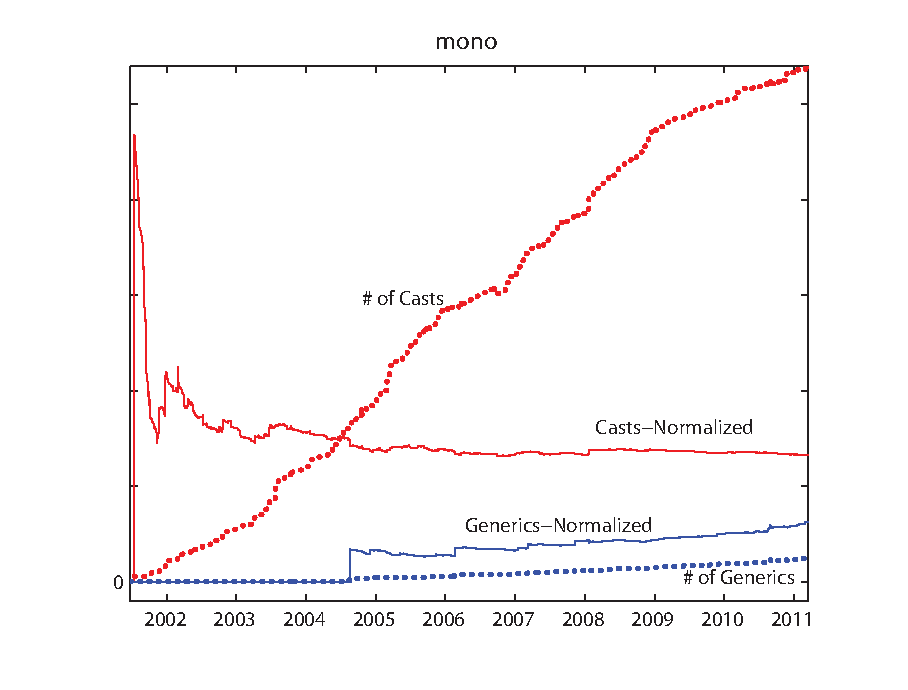
\includegraphics[width=0.7\textwidth]{fig3_mono_1016.eps}
\end{center}
\vspace{-25pt}
\begin{center}
\setlength{\tabcolsep}{2pt}
\begin{tabular}{cc}
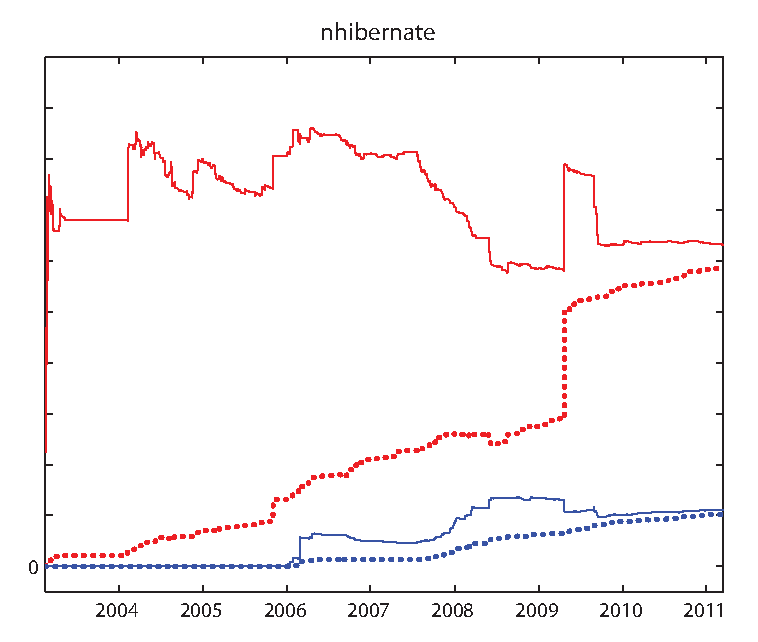
\includegraphics[height=3cm]{fig3_nhibernate_1016}&
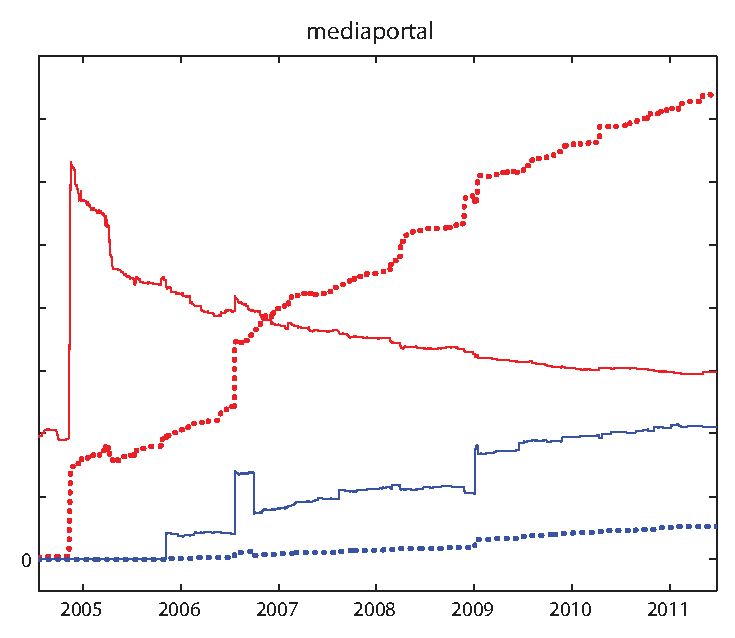
\includegraphics[height=3cm]{fig3_mediaportal_1016}
\end{tabular}
\end{center}
\vspace{-10pt}
\caption{Casts and parameterized types over time}
\vspace{-10pt}
\label{fig:cast}
\end{figure*}



Looking at Figure~\ref{fig:cast}, we observe the following: 

\begin{itemize}
\item The normalized value of casts tends to decrease consistently 
over time after a period of initial fluctuation.
%[FSE_review]
In some cases there are fluctuations in the middle of the graphs. 
For example, 
the \textit{nhiberate} project has a big jump of the normalized 
value of casts in the middle of 2009 due to unusually high usage of casts and 
the \textit{mediaportal} project has a small jump in the middle of 2006.
However, the overall decrease in casts does not appear to be directly related to generics,
since the normalized value of casts tended to decrease over time
for all projects, regardless of whether or when generics were introduced.

%although its value fluctuates in the initial stage.
%We note that 
%One reason may be that 
%a type cast is not limited to an explicit conversion of the operation related to raw types.  
%because it is an absolutely indispensable operation to the program.

\item The normalized value of generics tends to increase over time.
Nine projects show the number of generics increases monotonically, 
while the other projects show the number of generics increases steadily
with occasional, small drops in the number of generics. 
%while the other projects show the number of generics increases steadily 
%6 projects show the number of generics increases steadily but have some decline in the middle. 
%and 5 projects show the number of generics increases with marked decline.    
% EMH: it's simpler, but now it's contradictory. it says the number of generics both increases and decreases. how can it be both?
% also, try to be more objective than "barely noticable"

% 15 projects increase monotonically, Of those, 6 projects have small decrease.
% 5 projects (out of 20) have large decrease.    
%The number of generics increases consistently over time for all projects.
%Figure \ref{fig:raw_para} shows the number of generics more clearly.
%The normalized value of generics increases overall after introducing generics. 
  
%Although the normalized value of casts fluctuates in the initial stage, its value decreases consistently over time.
%\item The normalized value of casts decreases while that of generics increases. 
%\item The growth rate of the number of casts is less than that of program size.
%In contrast, the growth rate of the number of generics is higher than that of program size.
\end{itemize}

In addition to these general trends, several specific trends 
suggest that some relationship between generics and casts exists
in several projects.
For example, the \emph{nhibernate} project shows that 
the normalized value of generics spikes from mid of 2007 to mid of 2008
while the normalized value of casts sharply decreases. 
%At the same period time, as we showed in Figure \ref{fig:raw_para}, 
%the number of parameterized types sharply increases while the number of raw types decreases. 
%These results indicate that  
We found such inverse relationships in several other projects as well, including
%in several projects that 
%the rising normalized value of generics reduces the normalized value of casts.
%In \emph{nhibernate}, the normalized value of generics sharply increases from mid of 2007 to mid of 2008
%while the normalized value of casts sharply decreases.
%The number of parameterized types sharply increases  while the number of raw types decreases in Figure \ref{fig:raw_para}.
%We found this inverse relationship in several projects: 
\emph{cuyahoga} between December 2007 and January 2008, 
\emph{ccnet} between March 2009 and April 2009, 
and \emph{mono} in the middle of 2004.
A total of 8 out of 19 projects which used generics %(\emph{log4net} did not use generics) 
show this sharp inverse relationship at some point in their histories. 
% 8 projects: jayrock, cuyahoga, ccnet, mono, mono-tools, nhibernate, monodevelop, tomboy.
At least for these projects, this implies that an 
increase in generics leads to a decrease in casts.
However, evidence exists for the opposite case,
with 4 projects showing both casts and generics increased concurrently at some point.
%However, 4 projects showed sharp direct relationships at some point,
%where both casts and generics increased concurrently.
% 4 projects: ankhsvn, mediaportal, nasa-exp, sgdk2

%Besides observable data characteristics,
%start after generics
%we assess how well the relationship between generics usage and casts usage by spearman's rank correlation coefficient.
%We note that four of the projects (\emph{mediaportal}: -0.88, \emph{monodevelop}: -0.89, \emph{banshee}: -0.77, and \emph{cuyahoga}: -0.76)
%show a strong negative relationship (between -0.7 and -0.1) and
%three projects (\emph{nhibernate}: -0.66, \emph{ccnet}: -0.58, and \emph{lucene.net}: -0.67) show a mild negative correlation (between -0.4 and -0.7).
%On the contrary, two projects (\emph{sdgk2}: 0.76 and \emph{zedgraph}: 0.77) show a strong positive correlation (between 0.7 and 1.0)
%and two projects (\emph{Castle}: 0.67 and \emph{beagle}: 0.52) show a mild positive correlation (between 0.4 and 0.7).


%Overall,
%the ratio of the total number of reduced casts due to the increased generics may be surprisingly low while the number total of casts is very large
%because a type cast is not limited to raw types.
%most of projects do not have a strong reverse relationship between the use of casts and the use of generics.
%However, the number of used parameterized types may have the effect on the number of reduced casts because generics replace explicit type casts.
%Thus, the data and our analysis indicate that \textbf{C\# generics do not support Hypothesis 1}.




%start from the first
Besides visual inspection of the data,
we assessed the strength of the relationship 
between generics and casts using Spearman's rank correlation coefficient~\cite{spearman_rank}.
For example, if Spearman's coefficient is a negative value, 
then an increase in generics is correlated with a decrease in casts (an inverse correlation).
Otherwise, it is a direct correlation. 
%If Spearman's coefficient is positive, then an increase in generics correlates with an increase in casts (a direct correlation).
Based on our research question, we may expect that most projects exhibit an inverse correlation.



\begin{table}
\scriptsize
\begin{center}
 \begin{tabular*}{6.77cm}{|c|c|lr|} 
\hline
\multicolumn{2}{|c|}{\textbf{Relationship}}  & \textbf{Projects} & \textbf{Value} \\ \hline \hline
\multirow{5}{*}{direct} & \multirow{1}{*}{strong [0.7,1)} 
%& sdgk2 & 0.90 \\
  & zedgraph	& 0.82 \\ 
 \cline{2-4}
& \multirow{3}{*}{mild [0.4,0.7)} & beagle &	0.69 \\
 &  & Castle &	0.57 \\ 
 &  & nasa-exp &	0.44 \\
 \cline{2-4}
 & \multirow{3}{*}{weak} & smuxi	& 0.18 \\ 
\cline{1-1} 
\multirow{13}{*}{inverse} & \multirow{2}{*}{} & tomboy & -0.10 \\
& & lucene.net & -0.32 \\
\cline{2-4}
 & \multirow{5}{*}{mild (-0.7,-0.4]} & ccnet &	-0.48 \\
 &  & mono &	-0.56 \\ 
 &  & mono-tools &	-0.58 \\
 &  & jayrock &	-0.65 \\
 &  & ankhsvn &	-0.68 \\
  \cline{2-4}
 & \multirow{7}{*}{strong (-1,-0.7]} & cuyahoga &	-0.78 \\
 &  & nhibernate &	-0.79 \\ 
 &  & mediaportal &	-0.86 \\
 &  & boo &	-0.80 \\
 &  & f-spot &	-0.87 \\
 &  & banshee &	-0.87 \\
  &  & monodevelop &	-0.89 \\
 \hline \end{tabular*}
 \end{center}
 \vspace{-10pt}
  \caption{The Spearman's rank correlation coefficient (at right) for each project.}
  \vspace{-10pt}
\label{tbl:spearman}
\end{table}


Table~\ref{tbl:spearman} shows Spearman's rank correlation coefficient for each project. 
We note that 6 of the projects
%(\emph{nhibernate}, \emph{mediaportal}, \emph{monodevelop}, 
%\emph{banshee}, \emph{f-spot}, and \emph{cuyahoga})
show a strong inverse relationship and
5 projects
%(\emph{ccnet}, \emph{ankhsvn},\emph{ mono-tools}, \emph{mono}, and \emph{jayrock})
show a mild inverse relationship.
On the other hand, 2 projects 
%(\emph{sdgk2} and \emph{zedgraph})
show a strong direct relationship 
and 3 projects
%(\emph{Castle}, \emph{beagle}, and \emph{nasa-exp}) 
show a mild direct relationship.
%%%  
In short, 12 (63.1\%) out of 19 projects indicate an inverse relationship between the use of casts and the use of generics.
Seven out of the 8 projects that showed the sharp inverse relationship by our visual inspection
also show an inverse Spearman correlation.   
Of those 7 projects, the relationship was strong for both \emph{nhibernate} and \emph{cuyahoga}.




%We note the total number of casts is very large
%because, as we earlier note, a type cast is not limited to raw types.
%However, the number of used parameterized types may have the effect on the number of reduced casts because generics replace explicit type casts.

Overall, our results suggest that \textbf{generics reduce casts in C\#}.
This conclusion about C\# generics is the same as our findings
for Java~\cite{java_generics_ese}. 
Similar to Java, data from a small number of projects suggests that
more generics sometimes coincides with more casts; further research
is necessary to reconcile our research question with these outliers.

%One limitation of our analysis is that our analysis is coarse-grained.  
%In future work, a fine-grain analysis can identify individual 
%casts that were removed due to using generics 
%and compare that with other contexts for removal.


%%%%%%%%%%%%%%%%%%%%%%%%%%%%%%%%%%%%%%%%%%%%%%%%
%%%%%%%%%%%%%%%%%%%%%%%%%%%%%%%%%%%%%%%%%%%%%%%%
\subsection{RQ2: Do generics prevent code duplication?}
\label{subsection:generics_code_duplication}

%\textbf{Hypothesis 2} - Introduction of user-defined generics classes reduce code-duplication. \\
%Java support Hypothesis 2. \\
 
To determine whether generics prevent code duplication (RQ2),
we analyzed the 20 projects in two different ways.
First, we determined how many unique type arguments are used
for each generic type.
Second, we estimated how many lines of code were
saved by using generics.

%Generic classes, declared by parameterized types, in C\# must be parameterized type; dual types(either raw or parameterized types such as Queue, SortedList, and Stack) are not allowed. C\# developer may intend multiple types for each generic class in case of generic classes; code duplication could be avoided. We estimate how many code duplication could be avoided by the number of unique parameterizations.

% unique_parameterization data
%1	152
%2	63
%3	25
%4	9
%5	7
%6	5
%8	4
%9	3
%10	1
%11	1
%12	1
%17	2
%23	1
%30	1
%total : 275

We first measure how many unique type arguments are used for each generic type
defined in a project.
%Boo: 8 different generic type, 3 one type argument
There are 283 different generic types defined by developers at the 
latest point of development in all projects combined.
The type that facilitated the most reuse was 
\texttt{IEquatable} in \emph{mono}, which was 
parameterized with 30 different type arguments.
However, \emph{most} generic types were instantiated only
once; 155 generic types (54.7\%) are parameterized with
only one type argument.
This number is much higher than in Java, where the percentage
of generic types parameterized with only one type argument 
was 38\%~\cite{java_generics_ese}.

%Donghoon: remove a histogram of number of unique...for space
%The distribution of the number of unique parameterizations 
%is shown in Figure~\ref{fig:unique_para}.

%\begin{figure}[!ht]
%\centering
%\includegraphics[width=2.4in]{fig2_distribution_user_defined0920.eps}
%\caption{A histogram of number of unique parameterizations of developer defined generic types.}
%\label{fig:unique_para}
%\end{figure}

%because generics permit common parameterized types such as \textless S, T\textgreater \ which will be replaced by specific types such as \textless int, int\textgreater \ or \textless double, double\textgreater
%when generics are instantiated.
%By reducing code duplication with generics, a program prevents general negative effects of duplicated codes such as code bloat and software maintenance (e.g. fixing copied bugs).
%methodology

We next estimated how many lines of code were saved by using generics.
To answer RQ2, we count how many different type arguments of each generic type is instantiated by a developer.
%the number of clones of \emph{user-defined}. measure the number of unique parameterizations 
%and estimate the number of clones.
We then take the number of unique parameterizations (P) of each
developer-defined generic type and count the lines of code (LOC) of each 
generic type at latest point of development.
We use the same formula that we used for Java~\cite{java_generics_ese} 
to estimate the total lines of duplicated code (D):

\begin{center}
\textbf{D = LOC * (P-1)}
\end{center}

\noindent
For example, suppose that there is a generic class defined by a developer 
called \texttt{MyStack<T>} that is 100 lines long, and that it
is instantiated with 3 different arguments in various places in the program: 
\texttt{MyStack<int>}, \texttt{MyStack<string>}, and \texttt{MyStack<double>}. 
Using the above formula, the total lines of duplicated code is 200.
Note that this is a rough estimate of duplication; realistically, 
a developer that does not use generics may be able to remove
duplication by creating a common superclass or extracting utility methods.


%Then, we estimate the potential faults with an error constant (K) in the code in this manner: E = D * R * K.

%analyze
% unique_parameterization data
%1	152
%2	63
%3	25
%4	9
%5	7
%6	5
%8	4
%9	3
%10	1
%11	1
%12	1
%17	2
%23	1
%30	1
%total : 275
We estimated the number of lines of code in all generic types by calculating 
the mean lines of code for the top 20 developer-defined generic types,
ordered by the number of unique type instantiations (the mean is 674 lines).
We did this estimation because our framework did not automatically calculate the 
number of lines of code for all developer-defined
generic types.
Next, across all 20 projects, we found that generic types have a total of 633 
distinct parameterized types instantiated from 275 generic types.
This indicates that 358 class and interface duplicates were avoided.  

Using our formula, we estimate that 241,292 lines 
of duplicated code would be avoided,
which is 4.0\% of the total number of lines of code 
in all 20 C\# projects.
This percentage of C\# code duplication prevention 
is much higher than the percentage of Java code duplication prevention (0.02\%)~\cite{java_generics_ese}.
%which is calculated from the total LOC (548,982,841 lines) divided by an estimated duplicated code (109,816 lines and 176 mean LOC) 
%===mono===========
%1	59
%2	21
%3	6
%4	5
%5	1
%6	1
%8	1
%11	1
%12	1
%23	1
%30	1
%Total :98
%====================
%[JOT_review]
One reason is that the mean LOC of C\# generic types (674 lines) were about twice that of Java generic types (378 lines).
Another reason is that the \emph{mono} project tended to make unusually 
heavy use of large generic types, and skewed the result somewhat.
% tended to 
% which implemented the generics class library for C\# 2.0 \cite{c5_generic}: 
% (1) it has the source code of the generics library in C\# 2.0 such as \texttt{IEquatable} and \texttt{IComparable} 
% so it includes more number of \textbf{p-user} than other projects.
% It has 234 (37.0\%) out of 634 variations 
% and prevents 136 classes and interfaces (38.0\%) duplication,
% and 
% (2) some generic types such as \texttt{HashedLinkedList} and \texttt{TreeSet} have more than 3,000 LOC.
If we exclude the \emph{mono} project from the estimation of the code duplication, 
we estimate that 24,198 lines (0.8\%) of duplicated code would be prevented.
%0.8% (24198/2889700)
Interestingly, this percentage is still more than an order of magnitude higher than 
the Java percentage (0.02\%), even though 
the mean LOC (109 lines) of the C\# generic types defined by developers 
is now three times smaller than that of Java. 

%EMH I think the following can be inferred
%This indicates that the percentage of the number of variations of \textbf{p-user}, instantiated from C\# generic types defined by developers, 
%is much higher than that of Java generic types defined by developers.  

Overall, our results suggest that \textbf{C\# generics reduce duplication}.
Although the total amount of duplication prevented is small relative
to the size of the projects,
more duplication is prevented in C\# projects than in Java projects.

%A limitation of our analysis is that it only applies to code duplication internal to a project.
%One factor that is not accounted for is that some generic library classes may be intended for client use.
%In those cases, we may be underestimating the amount of code duplication reduced.

%%%%%%%%%%%%%%%%%%%%%%%%%%%%%%%%%%%%%%%%%%%%%%%%%%%%
\subsection{RQ3: Are generics used widely by developers?}
\label{subsection:generics_by_developers}
%%%%%%%%%%%%%%%%%%%%%%%%%%%%%%%%%%%%%%%%%%%%%%%%%%%%



Recall that C\# generics are used by most 
projects in Section~\ref{subsection:projects}.
Specifically, only one project never used generics at all,
and 11 projects have higher usage of parameterized types 
than that of raw types.
%To use a new feature in open source projects, community consensus may be required by a group.
%This processing may encourage group members to use a new feature.
But how do different developers use generics?
%To investigate how many C\# developers use generics,    
To evaluate RQ3,
we first examined commits that create or modify generics (parameterized types, 
generic type declarations, or generics method declarations) and
those that create and modify raw types.  
We term these commits ``associated'' with generics or raw types, respectively.
In total, 663 developers made 109,714 commits to the projects. 
Of those developers, 219 used generics (34.3\%),  
332 developers used raw types (52.0\%), 
and 182 developers used both generics and raw types (28.2\%).
For each developer, the average number of commits that introduced or modified 
parameterized types is 40 commits and 
the average associated with raw types is 29 commits.
The total number of commits associated with parameterized types is 8,782;
the total number associated with raw types is 9,527.
The data suggests that a smaller number of developers use
%(create or modify)
parameterized types more frequently 
than the larger number of developers use raw types.

% we observed that there was 
%a smaller pool of developers who used parameterized types exclusively, in comparison to developers who used both or none.
%In this section, we evaluate RQ1, whether individual developers widely use generics. 
%
%the number of developers using raw types is larger than that of developers using generics,
%but the number of raw types used by developers is smaller than that of generics used by developers.
%Thus, we analyze who uses generics in the projects after adopting generics
%in order to see how generics are used widely in C\# projects.

\begin{figure*}[ht]
\centering
\begin{center}
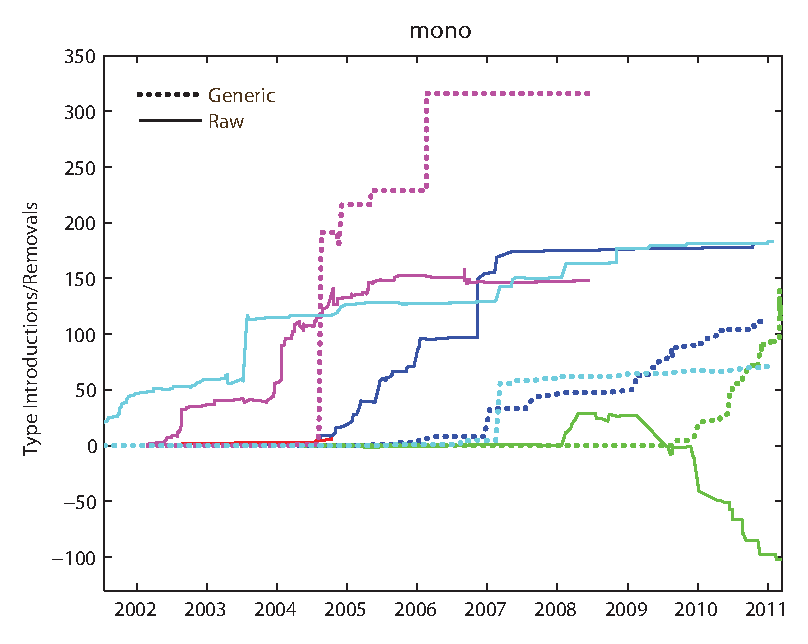
\includegraphics[width=0.7\textwidth]{fig5_mono.eps}
\end{center}
\vspace{-15pt}
\setlength{\tabcolsep}{2pt}
\begin{center}
\begin{tabular}{cc}
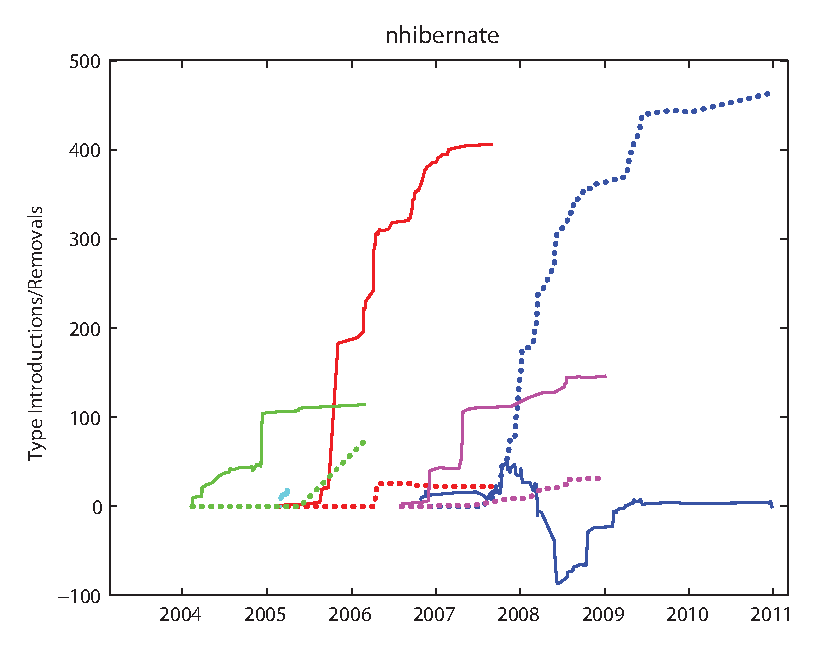
\includegraphics[height=3.5cm]{fig5_nhibernate.eps}&
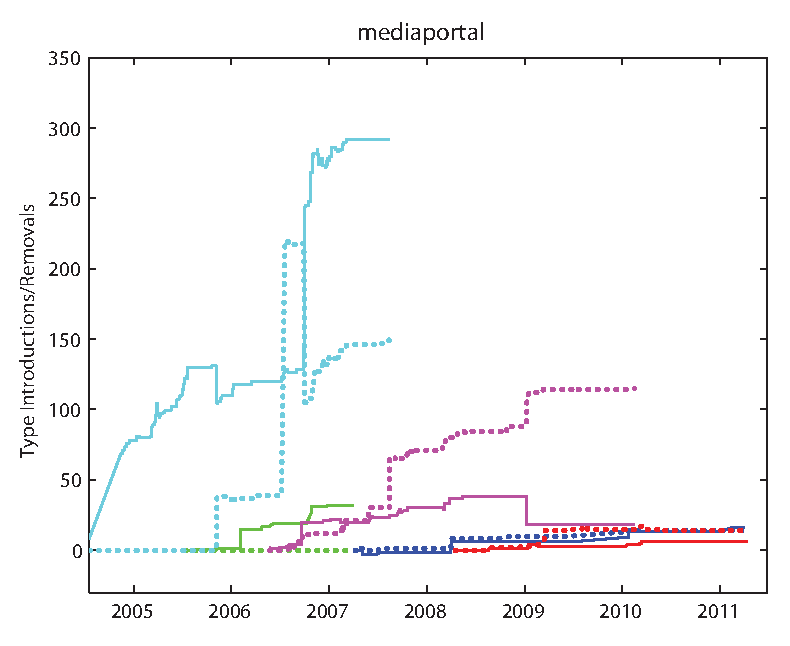
\includegraphics[height=3.5cm]{fig5_mediaportal.eps}
\end{tabular}
\end{center}
\vspace{-10pt}
\caption{Individual developers' introduction and removal of parameterized types}
%\vspace{-10pt}
\label{fig:contributors}
\end{figure*}


%\begin{figure*}[!ht]
%\begin{center}$
%\begin{array}{ccc}
%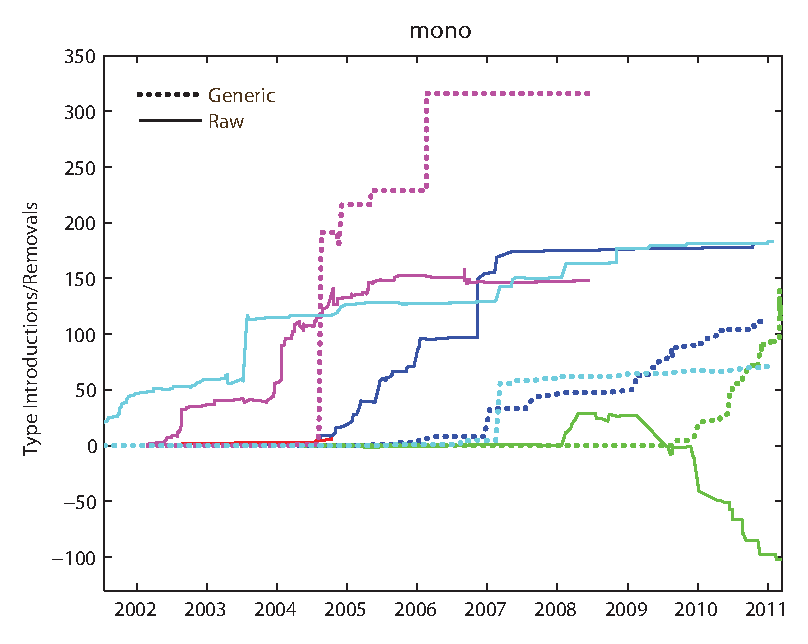
\includegraphics[width=0.3\textwidth]{fig5_mono.eps} &
%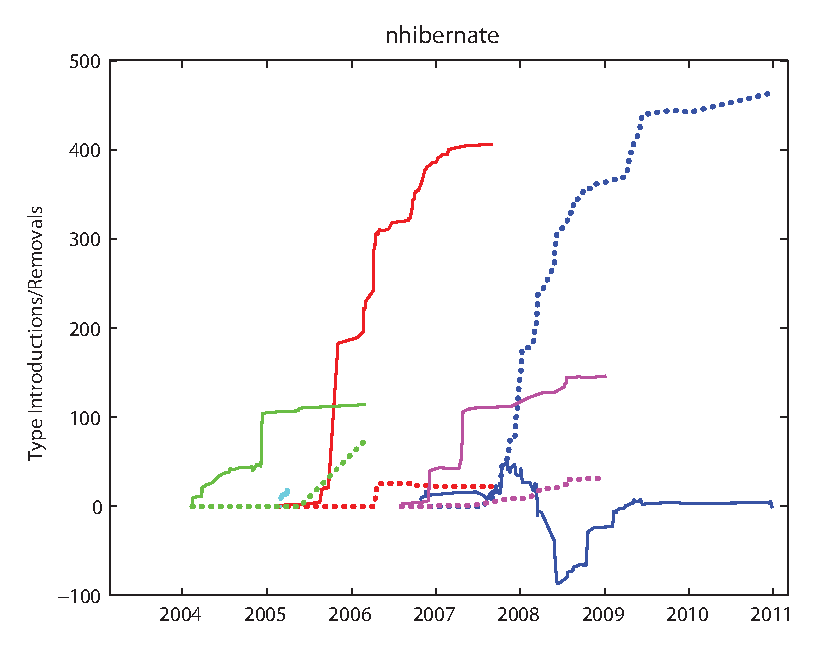
\includegraphics[width=0.3\textwidth]{fig5_nhibernate.eps}&
%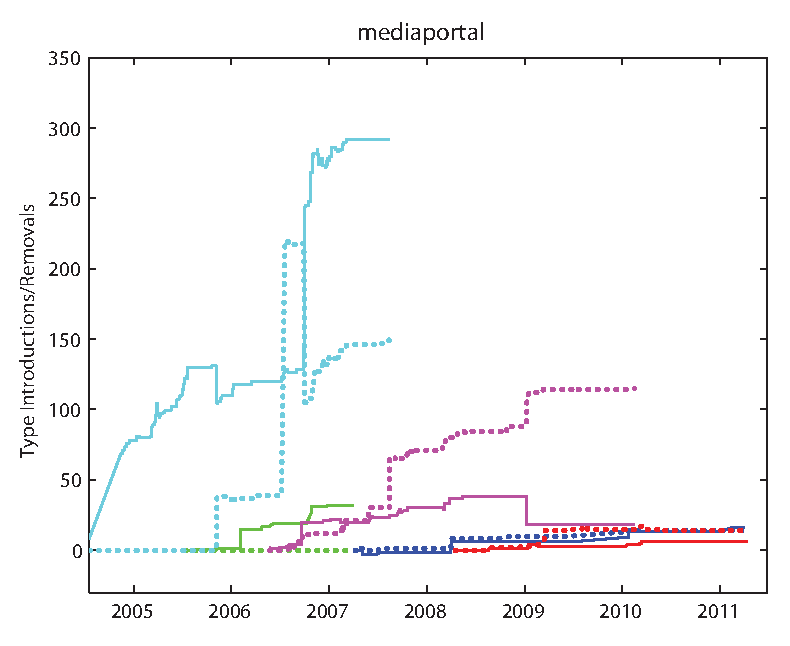
\includegraphics[width=0.3\textwidth]{fig5_mediaportal.eps}
%\end{array}$
%\end{center}
%\vspace{-20pt}
%\caption{Individual developers' introduction and removal of parameterized types.}
%\vspace{-10pt}
%\label{fig:contributors}
%\end{figure*}


Figure \ref{fig:contributors} shows the introduction and removal of both raw and parameterized types
by the most active developers per project.
%[FSE_review]
By ``most active'', we mean up to 5 developers who made the most commits
and, as a group, committed more than 50\% of the total commits.
A dashed line represents the number of parameterized types while a solid line represents the number of raw types.
An upward sloping line represents the introduction of parameterized types, while a downward
sloping line represents removals.
Pairs of lines with the same color denote the same developer.
%In the \emph{mono} project 
%which has higher number of raw types than that of parameterized types,  
%three developers show higher usage of raw types, while the other two developers show higher usage of parameterized types.
%In the \emph{nhibernate} project,
%four developers show higher usage of raw types, whereas only one developer (\textcolor{blue}{blue}) used higher usage of parameterized types.
%In the \emph{mediaportal} project,
%three developers show higher usage of raw types and two developers used more parameterized types than that of raw types.
As was the case with Java projects, 
we observe that one or two developers show higher usage of 
generics in the projects as shown in Figure~\ref{fig:contributors}.
This pattern was observed in the other C\# projects 
such as \emph{ankhsvn}, \emph{banshee}, \emph{ccnet}, \emph{f-spot}, \emph{jayrock}, and \emph{smuxi}.
%ankhsvn: 1,  banshee: 2, ccnet: 1, f-spot: 2,  jayrock: 1, smuxi: 1
%   
% 
%In the other projects, we found that several developers in each project used much more parameterized types than raw types.
%Fisher's exact test : http://faculty.vassar.edu/lowry/tab2x2.html
%example : http://www.medcalc.org/manual/fisher_exact_test.php

Based on this visual inspection, it appears that some developers dominate generics usage.
To determine if there is a developer who uses generics significantly more 
on average than other developers, 
we conducted Fisher's exact test~\cite{Fisher-exact-test} 
(applying Benjamini-Hochberg procedure for p-value correction to control the false discovery rate~\cite{Benjamini95})   
for the top five developers, ordered by the number of parameterized types that developer contributed.
We excluded 9 projects that had fewer than 3 developers and one project that
did not use generics.
We used the ratio of raw types to parameterized types at the latest 
point of development for each developer for the table values in Fisher's exact test.
%we do not use the number of the two types 
%
In this test, we compared
the ratio from the the developer who contributed the most
parameterized types against the ratio from the other four developers.  
If all p-values are smaller than .05 for each developer, 
the top developer uses generics significantly more than 
the other developers.

The result was that there was no developer that used generics more than the others to a statistically
significant degree ($p > .05$) in the following 10 projects: 
\emph{nhibernate}, \emph{mono}, \emph{monodevelop}, \emph{mediaportal}, \emph{ankhsvn},
\emph{banshee}, \emph{f-spot}, \emph{mb-unit}, \emph{mono-tools}, \emph{tomboy}.  
%TODO DH what about the other 1 project?
This means that, for these projects, although one developer may have used generics
more than the others, that person did not do so to a level enough to ``stand out'' and other
developers used parameterized types about as much as the top developer used them.  


Overall, our results indicate that \textbf{C\# generics are used by a small pool of C\# developers}.
Unlike Java generics, 
%[JOT_review]
%where a single ``champion'' emerged who used generics more than other developers, 
where a single developer in a project tended to use parameterized types significantly more than the other developers,
in these C\# projects, several developers per project made significant use of parameterized types.

%In \cite{java_generics_ese}, the answer of Research Question 1 is \emph{No} and a champion exists in Java projects. On the other hand, we expected that more developers use generics in C\# projects since the usage of parameterized types is higher in most of C\# projects in Figure \ref{table:20projects}.
%In subsection developers \ref{subsec:developers} , however, the data shows that fewer developers use generics more frequently. Although C\# projects do not support Reserach Question 1, the developers who know how to use generics use more generics rather than the developers using raw types.
%Accordingly, we examine the introduction and removal of parameterized types by developers over time whether there is a champion or not.
%Figure \ref{fig:contributors} shows the introduction and removal of both raw and paramterized types with top five contributors by the number of paramterized types.
%A dashed line represents the number of paramterized types while a solid line represents the number of raw types.
%Pairs of lines with the same color denote the same contributor.
%In mono project,
%the usage of predominant raw types,
%three contributors show the higher usage of raw types and the other two contributors show the higher usage of parameterized types.
%The downward slope of a solid line indicates that a contributor removed raw types after the mid of 2009 while introducing parameterized types.
%In nhibernate project,
%two contributors show the higher usage of raw types and two contributors show the higher usage of parameterized types.
%The one contributor just started using generics.
%In monodevelop project,
%all four contributors show the higher usage of parameterized types as this project has the higher usage of parameterized types.
%We noted that there is a champion at each project.
%In order to use C\# generics, C\# developers should know the kind of p-only and p-choice in either collection or generic namespace.
%Otherwise, C\# developers may be in a state of confusion while they meet generics in their project.
%That could be a challenge for C\# developers to learn the generic feature
%so they may recognize the benefits of generics programming well and intend to reflect those advantages to the projects.
%These conditions may give a hint to language designers regarding the importance of implementing new language features.

%%%%%%%%%%%%%%%%%%%%%%%%%%%%%%%%%%%%%%%%%%%%%%%%%%%%%%%%%%%%%%%%%%%%%%%%%%%
\subsection{RQ4: Are there large-scale conversions from raw types to generics?}
\label{subsection:covert_old}
%%%%%%%%%%%%%%%%%%%%%%%%%%%%%%%%%%%%%%%%%%%%%%%%%%%%%%%%%%%%%%%%%%%%%%%%%%%%

Despite the benefits that generics may have, 
developers may not convert old code using raw types to use generics.
On one hand, using generics may expose and correct dormant InvalidCastExceptions and
help reduce duplication in existing code.
On the other, developers may not migrate old code
because they do not want to risk changing old code that already works.
To evaluate whether developers perform such migrations (RQ4), 
we examined how many raw types are converted to parameterized types.

%which may be implemented complicatedly but is nevertheless \textit{bug-free code}.
%For example,  
%\texttt{SortedDictionary} (\textit{O}(\textit{log n})) in C\#2.0 can replace \texttt{SortedList} (\textit{O}(\textit{n})) in C\# 1.1.
%developers may take action to obtain fast insertion and removal of data.       
%Developers may make extra efforts to convert the existing code that is \textit{bug-free code} to new \textit{bug-free code}. 


%Java generics only show a few large-scale conversion efforts \cite{java_generics_ese}.
%C\# generics may even have a lower chance to convert raw types to parameterized types
%due to the different implementation of C\# generics,
%compared with Java generics as indicated in Section \ref{subsection:comparison}.
%For example,
%in C\# 4.0, 11 out of 40 classes from both Collections namespace and Collections.Generic namespace are the candidates for conversion.
%The efforts of conversion by C\# developers may be limited.

\begin{figure*}[ht]
\centering
\begin{center}
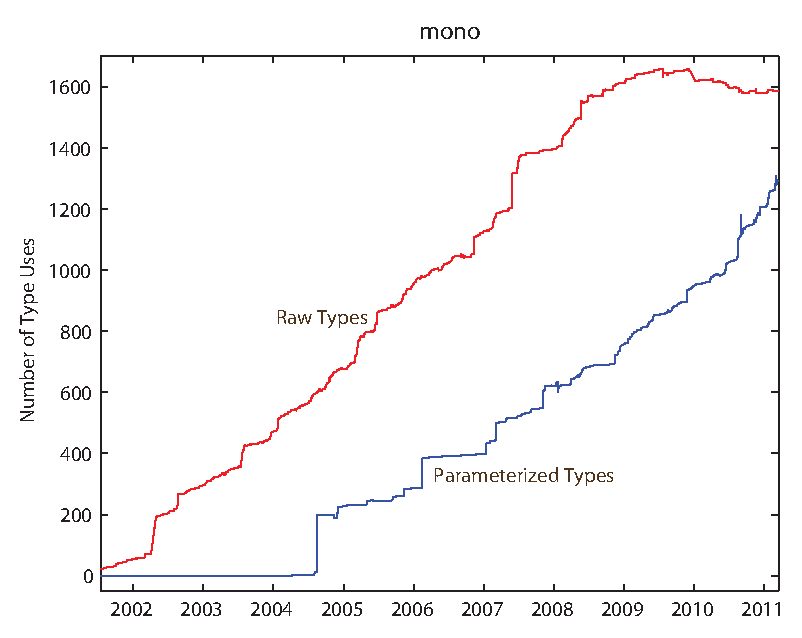
\includegraphics[width=0.7\textwidth]{fig4_mono_1213.eps}
\end{center}
\begin{center} 
\setlength{\tabcolsep}{2pt}
\begin{tabular}{cc}
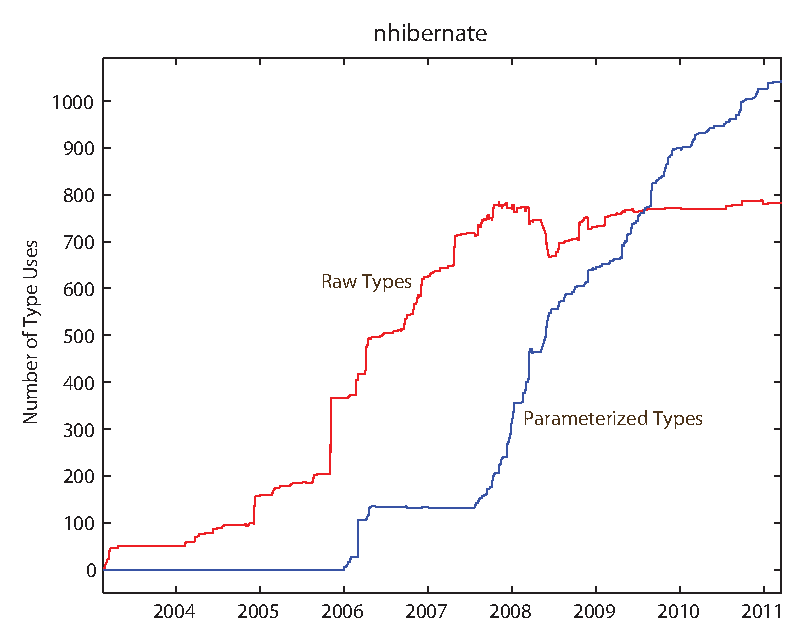
\includegraphics[height=3.5cm]{fig4_nhibernate_1213.eps}&
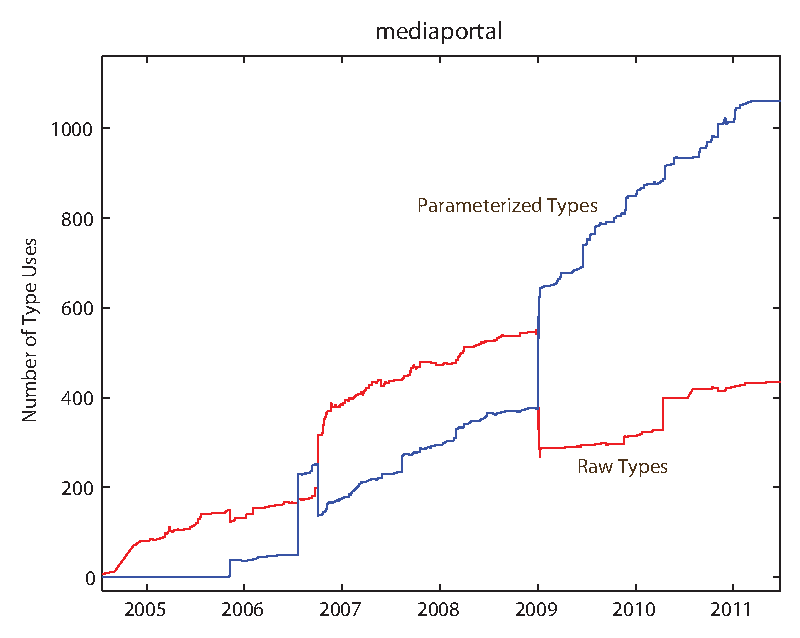
\includegraphics[height=3.5cm]{fig4_mediaportal_1213.eps}
\end{tabular}
\end{center}
\vspace{-10pt}
\caption{The number of raw types and parameterized types over time.}
%\vspace{-10pt}
\label{fig:raw_para}
\end{figure*}


%We suppose that any raw type is a candidates to be a parameterized type
%since the ratio of removed raw types before introducing generics is much less than that of removed raw types after generics.
%
%Java projects show a trace of conversion of raw to parameterized types, not a large-scale efforts \cite{java_generics_msr_2011}. What about C\# project? C\# generics can not have the whole types conversion; only dual types (p-choice and r-choice) can be exchanged. In C\# 4.0, 11 out of 40 classes from both Collections namespace and Collections.Generic namespace are the candidates for conversion. The efforts of conversion by C\# developers may be limited.
%
%We analyze the transition of the usage of raw types and parameterized types over time in Figure \ref{fig:raw_para}. On the x-axis of the figure is time. On the y-axis is the number of types. We also draw four extra lines for the detail transition of Dual and Single information, i.e., Adding p-choice and p-only is the number of parameterized types.
We begin with a visual inspection of the data.
Figure~\ref{fig:raw_para} shows the number of raw types and parameterized types over time for three projects.
%six lines; for dual types (\emph{p-choice} and \emph{r-choice}) and single types (\emph{p-only} and \emph{r-only}).
The \emph{mono} project shows a small conversion around January 2010,
and then a leveling off of raw types and a steady increase in the number of generics.
%More specifically, the number of \textbf{r-only} decreases while the number of both \textbf{p-choice} and \textbf{p-only} increase. 
%the number of raw types (solid blue) is higher than parameterized types (solid red) over time.
%After July 2009, the number of raw types remains more or less constant while the number of parameterized types is still increasing;
%this may be the evidence that the \emph{mono} project converts raw types to generics. 
%The number of \emph{r-only} (round dot blue) is much larger than the number of \emph{r-choice} (square dot blue).
%After introducing generics in July 2004, the number of parameterized types are also increasing continuously.
%The number of \emph{p-only} (round dot red) is also much higher than the number of \emph{p-choice} (square dot red).
%After July 2009, the number of raw types remains more or less constant while the number of parameterized types is still increasing.
%We can see a short downward slope of raw types while the number of parameterized types is increasing steadily.
Similarly, the \emph{nhibernate} project shows a conversion from December 2007 to June 2008,
with a similar leveling off of raw types and a steady increase in generics.
%The number of \textbf{r-choice} decreases sharply while the number of \textbf{p-only} increases sharply.
%the rate of the number of parameterized types is rising more rapidly than other projects after introducing generics in January 2006.
%The number of parameterized types is higher than that of raw types after June 2009.
%The number of \emph{p-only} is relatively higher than that of \emph{p-choice} while the number of \emph{r-choice} is much higher than that of \emph{r-only}.
%In \emph{monodevelop}, the number of parameterized types is much higher than that of raw types.
%The number of parameterized types are increasing steadily after introducing generics in June 2006
%while the number of raw types are rarely increasing after April 2008.
The \emph{mediaportal} project shows a large scale conversion effort in January 2009,
where more than 250 raw types are converted to parameterized types.
Unlike the other two projects, all of the raw types from \texttt{System.Collections} were converted into 
their equivalent generic types from \texttt{System.Collections.Generic}.
%The \emph{ankhsvn} project shows a small conversion in April 2008.
 
We next estimate the number of conversions in each project.
In each revision, if the number and type of parameterized types added to a method in the
project equals the number and corresponding type of raw types removed in the same method, 
we count each raw types removed as a conversion.
%EMH the following seem redundant
%Because we found that a large number of conversions from raw types to parameterized types do occur in the same revision in C\# projects,
%we count the number of removed raw types in the revision where there are parameterized types added 
%after introducing generics in a project. 
%
%
%after manually examining \textquotedblleft generification\textquotedblright \ from revision information. 
%We note that this approach produces relatively higher number of \textquotedblleft generification\textquotedblright \ when compared with Java \textquotedblleft generification\textquotedblright \ Parnin \emph{et al.} used in \cite{java_generics_ese}
%because new generic collections in C\# 2.0 use different name. 
% To calculate the conversion ratio (generification; from raw types to parameterized types),
%we apply a more loosened generification function than the one used in \cite{java_generics_ese};
%we ignore revision information
%and only count the number of removed raw types and the number of added parameterized types after introducing generics in a project.
In \emph{mono}, 1,938 raw types are added, but only 120 (6.2\%) were converted.
In \emph{nhibernate} 235 of 1,072 (21.9\%) are converted and
in \emph{mediaportal} 324 of 885 (38.9\%) are converted.
Although the \emph{tomboy} shows the highest conversion rate (72.4\%), 
the project only had 29 raw types in total.
In total, 6 projects show more than 10\% conversion, 
%tomboy, anksvn, mono-tools, mediaportal, nhibernaet,smuxi
6 projects have between 0\% and 10\% conversion,
%castle, mono,f-spot,monodevelop,ccnet,banshee
and 7 projects have no conversion at all.
%beagle,cuyahoga,jayrock,lucene,nasa,sgdk2,zedgraph
Across all projects, about 14\% of raw types were converted.
In comparison, in Java that number was about 8\%, although
the difference between Java and C\# was not statistically 
significant (Mann-Whiteney U-test, p\textgreater .05).

Overall, our reesults suggest that 
\textbf{most projects do not perform significant generic migrations in old code},
although we do observe a few large-scale efforts in some projects.
This finding is consistent with our findings for Java~\cite{java_generics_ese}.
%Threats to Validity
%A potential threat to the validity of this analysis is that 
%our heuristic for identifying conversions from raw types to generics
%may have counted some changes as migrations when they were not
%and vice versa.  However, we evaluated this heuristic in previous
%work and found that it was in fact quite precise~\cite{java_generics_ese}.

%Overall, . This means that C\# developers may not have a chance to convert raw to parameterized types.
%Thus, we conclude that \textbf{most projects do not indicate a large-scale conversion efforts for old code although we do see a few large-scale conversion efforts for raw types}.

%\subsection{When generics are shown?}

%To know how soon developers adopt generics feature in software projects,
%Parnin \emph{et al.} \cite{java_generics_ese} used the information of development environments, i.e.,
%IDEs and then concluded that generics adoption was not affected by IDE supports.
%On the other hand,
%C\# is closely dependent on IDEs;
%Microsoft Visual Studio (IDE from Microsoft) supports C\#.
%Generics are introduced in C\# 2.0, which is released with Visual Studio 2005.
%Thus, instead of investigating the correlation between generics adoption with IDE support for generics,
%we trace how soon generics are adopted in a project; when the first generic has been shown in a project.

%Table \ref{table:20projects} shows the date when the first parameterized type is shown in a project.
%Although we have not found yet the information when C\# 2.0 (Visual Studio 2005) has been used at each project for using generics,
%the \emph{mono} project even used generics before generics were officially released just like FindBugs java project.
%The \emph{lucene.net} project shows 1st P-type in June 2008, which is the very last.
%We note that the time gap of the dates for 1st P-type among projects is around 3 years.
%In the future work, we plan to investigate what factors affect the decision of when to begin using generics.


%Most of C\# developers prefer IDEs.
%For example, Visual Studios offer numerous features that make programming endeavors much simpler.
%On the other hand, few of C\# developers would deny IDEs since IDEs alone often do not provide access to all aspects of the underlying compiler.
%For example, Visual Studio 2005 does not support the generation of multifile assemblies.
%Although we have not found yet the information when C\# 2.0 (Visual Studio 2005) has been used at each project for using generics,
%we know the time when the first generics has been appeared in the project.
%As IDE support is not a critical factor in Java \cite{java_generics_msr_2011}, .NET framework may not be a critical factor of using generics.
%The mono project even used generics before generics were officially released just like FindBugs java project. Table \ref{table:20projects} shows the information of the first parameterized type.
%Our analysis indidates that \textbf{generics support in the IDE does not influence adoption}.
%As the future work of Java, we should also answer to the question, what factors affect the decision of when to begin using generics ?


%\section{Distinct characteristics of C\# generics}
%\label{section:distinctive_characteristics}

%We analyzed the distinct characteristics of C\# generics.
%Section \ref{subsection:generics_performance} investigates the benefit of C\# generics that C\# generics improve performance.
%Section \ref{subsection:prefer_var_type} investigates 
%the effect of the usage of C\# generics by the \texttt{var} type which is used as the implicit generics type declaration.  



\subsection{RQ5: Do generics improve performance?}
\label{subsection:generics_performance}

As we explained in Section~\ref{subsection:comparison},
generics may improve the overall performance of a project
because when value types are used as generic type arguments,
values do not have to be converted to and from objects.
To estimate whether performance could actually be improved in
open-source C\# projects (RQ5), we analyzed how many value types 
are used as generic type arguments in a project. 

%%%%%%%%%%%%%%%%%%%%
%remove for space by Donghoon
\begin{figure*}[!ht]
\centering
\begin{center}
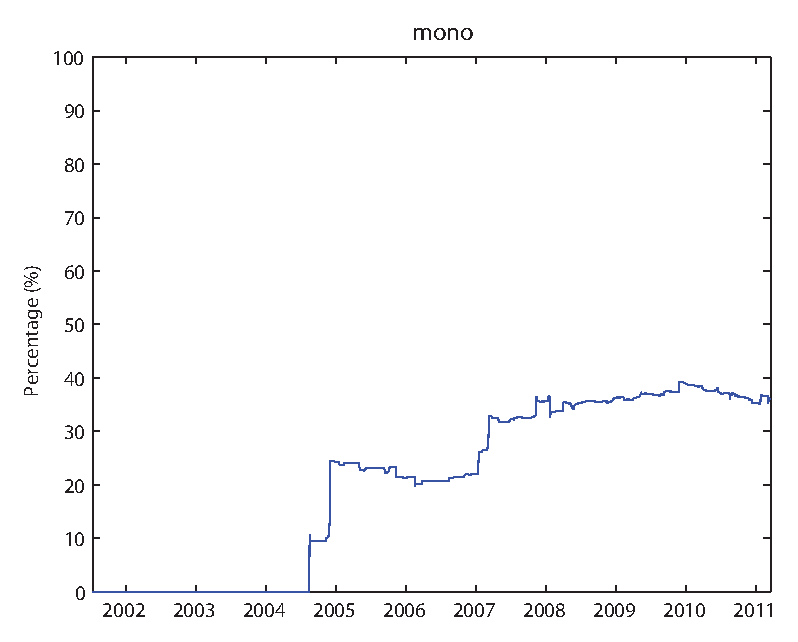
\includegraphics[width=0.7\textwidth]{fig6_mono_1213.eps} 
\end{center}
\vspace{-15pt}
\setlength{\tabcolsep}{2pt}
\begin{center}
\begin{tabular}{cc}
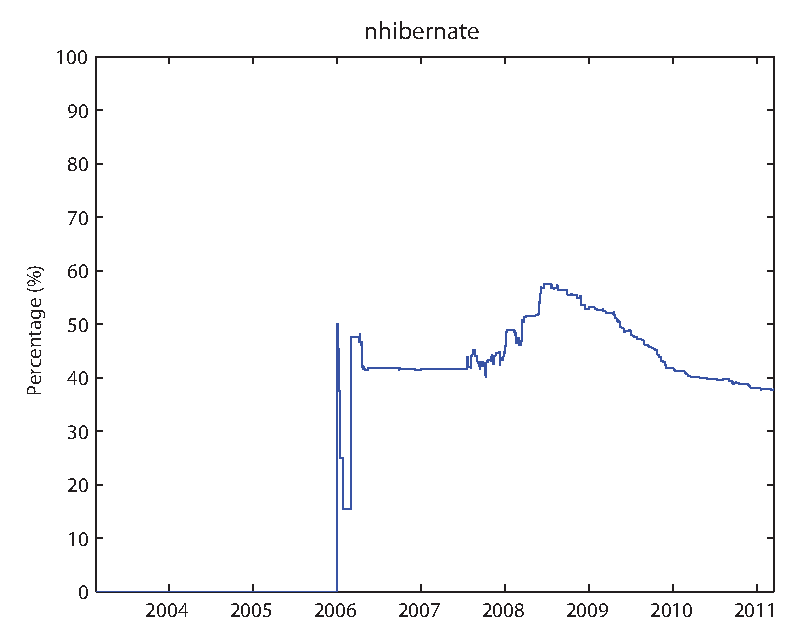
\includegraphics[height=3.5cm]{fig6_nhibernate_1213.eps}&
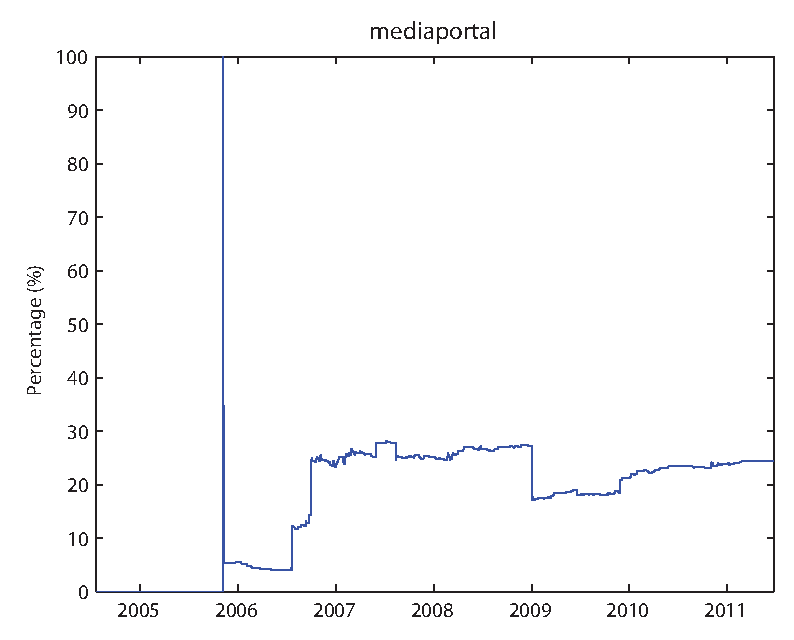
\includegraphics[height=3.5cm]{fig6_mediaportal_1213.eps}
\end{tabular}
\end{center}
\vspace{-10pt}
\caption{The percentage of value types used in parameterized types over time.}
\label{fig:performance}
\end{figure*}
%\vspace{-10pt}

Figure~\ref{fig:performance} shows the percentage of value types 
used in parameterized types over time for three projects. 
In total, 17 out of 19 projects that used generics
also used value types as generic type arguments.
Of those 17, value types were used in 35.9\% of parameterized types.
After the project introduces generics, over time the overall 
usage of value types in each project remains more or less constant 
above 30\% for most projects. 
%with Boo: 30.5%, before:30.4%
%(Figure~\ref{fig:performance}).
According to the performance comparisons performed by 
Kennedy and Syme~\cite{DBLP:conf/pldi/KennedyS01},
use of value types with generics can provide a significant speedup 
compared to \texttt{object} conversion.
For example, they showed that 
when \texttt{int} and \texttt{double} were used as generic type arguments 
in a small benchmark, they were able to achieve a speedup of
4.5 times and 5 times, respectively, compared to a similar benchmark
without generics.
%[FSE_review]
This indicates that the performance of C\# projects doubles while executing generic 
code that includes 30\% value types in parameterized types, 
which are 4.5 times faster than reference types. 
%as Kennedy and Syme implemented \textquotedblleft C\# stack\textquotedblright \ and \textquotedblleft Generic C\# stack\textquotedblright
%programs \cite{DBLP:conf/pldi/KennedyS01}   
%So we estimated performance improvement of generics codes used value types as generic type arguments 
%based on the processing overhead due to boxing and unboxing operation.
%Figure~\ref{fig:performance} shows the performance improvement based on value types over time. 
%The percentage of value types directly affects the performance improvement. 
%10 projects showed more than 45\% performance improvement while 2 projects showed less than 30\% performance improvement.
Overall, our results suggest that \textbf{C\#'s implementation of 
generics improve performance}.
% although it is limited evidence in \textbf{support of RQ5},
%since developers often use value types in with their generics.

%Threats to Validity
%The main limitation of our analysis stems from our static analysis of performance.
%There may be other conditions that mask or dwarf the performance gains from value types 
%during execution of the program.
%In the future, a dynamic analysis of these programs using their own unit tests would 
%allow us to more accurately measure what performance gain developers can expect from using generics
%with value types.

%To test H3, we analyze how the usage of C\# generics affects performance in a project.
%Assume that C\# generics are implemented in two cases: 
%(1) without performance gain for value types,
%and 
%(2) with performance gain for value types. 
%If C\# generics use value types as type arguments in a project, 
%C\# generics in the second case of the above assumption improve performance in a project 
%compared with the first case of the above assumption which C\# generics are implemented without performance gain for value types.
%The first case is the same as reference type since value types should be converted to reference type 
%when value types are placed in a generic type. 
%Thus, we can compare value types with reference types. 
%We do not consider that the application as a whole achieve improvements in performance as Lowy \cite{intro_CSharp_generics} showed.  
 
 
%We define the \textbf{performance index} which is 
%the relative ratio of the run-time overhead between value types and reference types. % which we call \textbf{performance index}.
%Table \ref{table:performance_ratio} shows \textbf{performance indices} which are used to estimate performance gain in a project.

%\begin{table}[h]
%\centering
%\begin{tabular}{|l||c|c|}
%  \hline
%   & \textbf{value types} & \textbf{reference types}    \\ \hline \hline
% \textbf{p-only} & 2.2  & 1.0\\
%  \textbf{r-only} & 1.0 & 1.0 \\
%  \textbf{p-choice} & 4.6  & 1.0  \\
% \textbf{r-choice} & 1.0 & 1.0  \\ 
% \textbf{p-user} & 1.5  & 1.0 \\
%  \hline
%\end{tabular}
%\caption{The performance indices for generics performance}
%\label{table:performance_ratio}
%\end{table}



%To calculate the \textbf{performance index}, the relative ratio of the run-time overhead,
%%when 
%a program executes a test code including generic types with a value type or a reference type. 
%%when upon executing 
%%measured by executing generic types
%%where generic types have generic type arguments between a value type and the \texttt{object} type. 
%when either a value type or the \texttt{object} type is used as generic type arguments,    
%between a value type and the \texttt{object} type, 
%which we call the \textbf{performance index}.  
%We consider the \texttt{int} type as value types and the \texttt{object} type as reference types.
%Experiments were conducted on Windows 7 Professional based on 2.60 GHz of Intel Core i5-2540M CPU and 8GB of memory. 
%We use the elapsed time to measure run-time overhead. 
%The following is the structure of the test C\# code. \\ % of \texttt{List<int>} to measure run-time overhead for value types: \\

%\noindent
%\footnotesize
%\texttt{\indent \textit{1}\indent\indent public static long TestCode(int howMany)\{ \\}			
%\texttt{\indent	\textit{2}\indent\indent\indent	\	Stopwatch sw = new Stopwatch(); \\}			
%\texttt{\indent	\textit{3}\indent\indent\indent	\	List<}\textbf{int}\texttt{> list = new List<}\textbf{int}\texttt{>(); //or %List<}\textbf{object}\texttt{> \\}
%\texttt{\indent	\textit{4}\indent\indent\indent	\	sw.Start(); \\} 
%\texttt{\indent	\textit{5}\indent\indent\indent	\	for(int i = 0; i < howMany ; i++)\{ \\}
%\texttt{\indent	\textit{6}\indent\indent\indent \indent			list.Add(i); // boxing \\}
%\texttt{\indent	\textit{7}\indent\indent\indent	\	\} \\}						
%\texttt{\indent	\textit{8}\indent\indent\indent	\	for(int i = 0; i < howMany ; i++)\{ \\}
%\texttt{\indent	\textit{9}\indent\indent\indent \indent			list.Remove(i); //unboxing \\}
%\texttt{\indent	\textit{10}\indent\indent\indent \}\\}			
%\texttt{\indent	\textit{11}\indent\indent\indent sw.Stop(); \\}			
%\texttt{\indent	\textit{12}\indent\indent\indent long duration = sw.ElapsedMilliseconds;\\}
%\texttt{\indent	\textit{13}\indent\indent\indent	return duration;\\}			
%\texttt{\indent	\textit{14}\indent \}\\} 
		
%\noindent
%\normalsize



%Table \ref{table:performance_ratio} shows performance indexes which are used to estimate performance gain in a project.

%Each generic type has two kinds of type arguments such as value types and reference types. 

%We use performance indexes to estimate performance gain in a project.
%To compute a performance index, we measure the run-time overhead due to the boxing and unboxing operations. 
%because value types do not require the boxing and unboxing operations when they are used as generics type parameters; 
%the other types do require the boxing and unboxing operations.


%To compute the \textbf{performance index} of \textbf{p-only},
%for \textbf{p-only}, 
%we measure the elapsed time from line\#~5 to line\#~10 when a program executes the test code.
%between \texttt{List<int>} for value types and \texttt{List<object>} for non-value types.
%The above test code is to measure the elapsed time of \textbf{p-only} for value types. 
%\texttt{List<int>} to measure run-time overhead for value types:
%For reference types of \textbf{p-only}, \texttt{List<object>} is substituted for \texttt{List<int>} on line\#~3.
%The result shows that the code of using \texttt{List<int>} is 2.2 times faster than the code of using \texttt{List<object>}.
%We use 2.2 as the \textbf{performance index} of \textbf{p-only} in value types and 
%1.0 as the \textbf{performance index} of \textbf{p-only} in reference types. 
%
%
% 
%as Kennedy and Syme implemented \textquotedblleft C\# stack\textquotedblright \ and \textquotedblleft Generic C\# stack\textquotedblright \ programs \cite{DBLP:conf/pldi/KennedyS01}.
%the \texttt{List<T>} class (which is the most used collection generic class overall in projects) in \textbf{p-only}
%shows that \texttt{List<int>} is 2.2 times faster than \texttt{List<object>};
%we use this value (2.2) as the performance index of \textbf{p-only} in \textbf{value types}.
%Moreover, 
%\texttt{Stack} class in \emph{r-choice} and \texttt{Stack<int>} class in \emph{p-choice} show the different performance (the elapsed time) when integer values are inserted and deleted;
%\texttt{Stack<int>} is 5.8 times faster than \texttt{Stack}.
%The other dual types (e.g. \texttt{Queue}---7.4 times and \texttt{SortedList}---3.2 times) shows the same results; 
%\emph{p-choice} is faster than \emph{r-choice} when the value types are used as generics type parameters.
%The elapsed times at each class are different so we take the mean value of \textquotedblleft most\textquotedblright \ used classes in a project; 
%\emph{p-choice} is 5.5 times faster than \emph{r-choice}.
%\textbf{Performance Index} denotes that a generics type has value types as its generic type parameters; 
%\textbf{Performance indices} of both \textbf{r-only} and \textbf{r-choice}  
%are set to 1.0 because there is no performance gain.    
%For \textbf{p-choice}, 
%we measure the elapsed time with two generic type arguments such as \texttt{int} and \texttt{object}
%as the above test code,  
%as the performance index of \textbf{p-only}. 
%The structure of the test code is the same as above code, 
%except line\# 3, 6, and 9 which are substituted with other generic types and methods related to those generic types.
%The results are as follows: \texttt{Queue}\---5.4 times, \texttt{Stack}\---3.7 times, and \texttt{SortedList}\---4.8 times.
%Such three collections are most used in projects.  
%We then take the mean value (4.6). 
%Thus, the \textbf{performance index} of \textbf{p-choice} in value types is 4.6 
%and 1.0 is the \textbf{performance index} of \textbf{p-choice} in \textbf{reference types}. 
%
%a generic type in \textbf{p-choice} with value types is 4.6 times faster 
%than a generics type without value types.
% 
% 
%a generics class in \textbf{p-choice} with value types (e.g. \texttt{int}) is 4.6 times faster 
%than a generics class without value types (e.g. \texttt{object}). 
%\textbf{lower} denotes that a generics type has no value types as its generics type parameters.
%\textbf{upper} denotes the case where generics can improve performance if there is a conversion from a raw type to generics:
%(1) \emph{r-choice} can be converted into \emph{p-choice} (performance index: 5.5) (e.g. from \texttt{Queue} to \texttt{Queue<int>}), 
%and (2) \emph{r-only} can be converted into \emph{p-only} (performance index: 1.2) (e.g. from \texttt{SortedList} to \texttt{SortedDictionary<int,int>}).
%For \textbf{p-user}, we implement two simple programs to measure the elapsed time: 
%\textquotedblleft C\# stack\textquotedblright \ and \textquotedblleft Generic C\# stack\textquotedblright \ 
%as Kennedy and Syme measured in \cite{DBLP:conf/pldi/KennedyS01}.
%The simple program is similar to \texttt{MyStack} in Section~\ref{subsection:general_terms},
%which is then implemented completely.    
%For \textbf{non-value types}, 
%we see that generics have no performance gain because raw types have no performance gain,
%as such all \textbf{non-value types} are set to 1.0 as the performance index.     



%We note that the \textbf{performance indices} we measured in Table \ref{table:performance_ratio} are based on a rough estimation.
%We only measured several generic types which are most used in projects and take the mean, 
%because we found that each type has a different \textbf{performance index} as   
%%(e.g. \texttt{Queue}, \texttt{Stack}, and \texttt{SortedList}) 
%\textbf{p-choice}.  
%we compare \texttt{int} type with \texttt{object} type for most used generics types in namespace and then take the mean value. 
%Thus, we again take the mean value among the most used generics types as we found in Section \ref{subsection:feature_breakdown}.  


%We implement two simple programs to measure the elapsed time: 
%C\# stack and Generic C\# stack as Kennedy and Syme conducted in \cite{DBLP:conf/pldi/KennedyS01}, 
%which are used to measure the elapsed time for \emph{p-user}.  
%First, we measure performance indexes To get index values, we measure run-time overhead, the elapsed time, in the following three cases.
%First, for run-time overhead due to boxing and unboxing,
% we implement two simple programs: C\# stack and Generic C\# stack, as shown in \cite{DBLP:conf/pldi/KennedyS01}, and then measure elapsed times, respectively.
%This value is used for default type in Table \ref{table:performance_ratio}.
%Second, we attempt to measure run-time overhead for \emph{r-choice} and \emph{p-choice} (e.g. \emph{Stack}, \emph{Queue}, and \emph{SortedList}).
%Third, we measure run-time overhead for \emph{r-only} and \emph{p-only}.
%We found that the elapsed times we measured are varying depending on what type parameters are used in a place of type arguments.
%We take the average from most used generics (e.g. \emph{ArrayList}, \emph{List}, \emph{Stack}, and \emph{Queue}) and type parameters (e.g. \emph{int} and \emph{string}).
%With these values of run-time overhead, we have actual performance indexes, i.e. relative ratios calculated from the elapsed times.
%If a developer use parameterized types, performance gain can be expected.
%Lower performance index means "no performance gain".
%Upper performance index means \emph{type} may be replaced with paramterized types for performance gain, i.e. p-choice and p-only.
%For example, \emph{dual} type can be used either p-choice or r-choice. If a developer uses p-choice, a project improves performance, otherwise, a project can not expect performance gain.

%the elapsed time for running on C\# generic stack as conducted in \cite{andrew_pldi_2001}; the elapsed time is to measure the overhead due to boxing and unboxing operation for the use of object type in a method or class declaration.
%Next we attempt to measure the elapsed time of generic collections to estimate how they have different performance since strongly typed collections provide better performance than non-generic strongly typed collections; the collections can be used either raw or parameterized type(e.g. Stack, Queue, and SortedList).
%We have found that the elapsed times we measured are various depending on what type parameters are used in a place of type arguments.
%We use the static program analysis instead of dynamic analysis because our analysis is based on each revision of the source code.
%Accordingly, we use the relative ratios taken from averages of each category.

%In addition, we calculate \emph{lower} bound and \emph{upper} bound based on actual performance indexes at every revision.
%The \emph{lower} bound means that generics may require overhead processing due to the use of object for \emph{p-only} and \emph{p-choice} or %\emph{r-only} and \emph{r-choice}.
%The \emph{upper} bound means optimal performance,
%which obtains when C\# developers may either use \emph{p-choice} instead of \emph{r-choice} or prefer generics collections rather than rawtype collections since some generics collections can replaced rawtype collections (e.g. \emph{List\textless T\textgreater ()} instead of\emph{ ArrayList()}).

%However, this is a rough estimation because of both difficulties of reflecting every single case (e.g. performance indexes for all collections in namespace based on all types) and the limitation of the static analysis. Table \ref{table:performance_ratio} shows the performance indexes based on relative ratios of generics performance.
%\begin{figure}[!ht]
%\begin{center}
%\includegraphics[width=2.6in,angle=90]{performance_index_1027_1.eps}
%\caption{The performance gain: 11 out of 19 projects show more than a 1.45 performance index in Unit,
%while 11 projects show less than a 1.25 performance index in Whole.}
%\label{fig:performance_bar}
%\end{center}
%\end{figure}


%Next, we apply the \textbf{performance indices} to the 20 selected projects.
%For example, assuming that there are two \textbf{p-only} with value types, two \textbf{p-choice} with reference types, and one \textbf{p-user} with %reference types in a project, 
%the performance obtained by generics is 1.48 calculated by (2.2 * 2 + 1.0 * 2 + 1.0 * 1) / 5. 
%In other words, generics would improve performance by 48\%. 
%We note that not all generic types instantiated in a program execute methods which are related to boxing and unboxing operations, 
%and there are limitations to our results due to the static program analysis that is performed without actual executing programs.
  





%Figure \ref{fig:performance_bar} show the performance gain for using generics with value types at the last point of each project. 
%The following is the explanation of each bar. 
%\begin{itemize}
%	\item \textbf{Unit}: the performance of generic types. 
%   We sum \textbf{performance indices} for each generic type, and then take the mean.
%   \item \textbf{Value Types}: the percentage of value types divided by all data types.
%   \item \textbf{Whole}: the overall performance.
%   We add up the \textbf{performance indices} for both generic types and raw types, and then take the mean. 
%\end{itemize}
% shows generics performance at the latest point of development for all projects 
%In Figure \ref{fig:performance_bar},
%(1) \textbf{Generics} denotes the performance of generic types in a project; 
%by summing performance indexes for each generics type, then taking the mean,  
%(2) \textbf{Value Types} denotes the ratio of value types divided by all data types in a project,
%and (3) \textbf{Overall} denotes the overall performance in a project;
%we add up the performance indexes for both generics types and raw types, then take the mean. 
%%
%%







%We observe \textbf{Unit} and \textbf{Value Types}:
%\begin{itemize}
%	\item 11 out of 19 projects %(the \emph{log4net} project has no generics) 
%	show more than a 1.45 \textbf{performance index} in \textbf{Unit};
%of those, the percentage of \textbf{Value Types} are higher than 30\%. 
%The \emph{beagle} project shows the highest \textbf{performance index} (2.0) and \textbf{Value Types} (83.7\%). 
% Overall, C\# generics improve performance more than 45\% in 11 projects. 


%	\item  4 projects such as \emph{sgdk2}, \emph{f-spot}, \emph{nasa-exp}, and \emph{zedgraph} show less than a 1.25 \textbf{performance index};
%of those, 2 projects such as \emph{nasa-exp}, and \emph{zedgraph} have no value types in generic type parameters.
%\end{itemize}
%\noindent
%(1) 11 projects out of 19 projects (\emph{log4net} project has no generics) show more than a 1.45 performance index in \emph{Generics};
%of those, the ratios of \emph{Value Types} are higher than 30\%. 
%The \emph{beagle} project shows the highest performance index (2.0) and \emph{Value Types} (83.7\%).  
%(2) 4 projects (\emph{sgdk2}, \emph{f-spot}, \emph{nasa-exp}, and \emph{zedgraph}) show less than a 1.25 performance index;
%of those, 2 projects (\emph{nasa-exp}, and \emph{zedgraph}) have no value types in generics type parameters.
%Next, we observe \textbf{Whole}:
%\begin{itemize}
%	\item 11 out of 19 projects show less than 1.25 \textbf{performance index}; 
%the \emph{sgdk2} project shows the lowest \textbf{performance index} (1.03) and \textbf{Value Types} (8.7\%) among the projects which used value types as generic type parameters.
%\end{itemize}
%(1) 11 projects out of 19 projects show less than 1.25 performance index; 
%the \emph{sgdk2} project shows the lowest performance index (1.03) and \emph{Value Types} (8.7\%) among the projects which used value types as %generics type parameters. 
%\noindent
%We note that the \textbf{performance index} of \textbf{Unit} is higher than that of \textbf{Whole}. 
%For example, in the \emph{beagle} project, the \textbf{performance index} of \textbf{Unit} (2.0) is much higher than that of \textbf{Whole} (1.16).  
%The mean of \textbf{Value Types} is 30.5\% for the projects which use value types. 
%We should not overlook expect that the performance gain from using generics may not affect if other programing operators   

 
  
  


 


%\emph{actual}, \emph{upper}, \emph{util}, and \emph{value types} 
%at the latest point of development for all projects; 
%\emph{util} is the ratio of \emph{upper} divided by \emph{actual}, 
%and \emph{value types} is the ratio of value types divided by all data types in a project.
%Only \emph{ankhsvn} project has over than 1.5 performance index; 
%most of the projects (15 projects) have less than 1.2 performance index. 
%Most of the projects show high percentage in \emph{util}; 11 projects shows more then 90\% util 
%while only \emph{zedgraph} project shows less than 80\% util.  
%Most of the projects show less than 20\% value types; 
%only two projects (\emph{ankhsvn} and \emph{lucene.net}) show more than 40\% value types. 
%It seems like that most projects have rarely chance to improve performance by generics because of the low ratio of value types.  


%Figure \ref{fig:performance} shows the change of performance gain over time by using generics with value types. 
%We %found an improved performance after introducing generics,
%and 
%noted that the percentage of value types directly affects the performance gain. 
%After an initial increase of the \textbf{performance index}, the \textbf{performance index} remains stable 
%as \textbf{Value Types} remain stable for most of the projects such as \emph{mono}, \emph{mediaportal}, and \emph{Castle}. 
%The \textbf{performance index} may not increase much further since the usage of value types remains stable in practice.  



%There are four lines: \emph{Best-case}, \emph{Actual}, \emph{Worst-case}, and \emph{Primitive-ratio}, which is added to show how many value types are placed as type parameters. Figure \ref{fig:performance_bar} indicates 
%The \emph{mono} project shows 1.5 actual performance index. Although the performance index of \emph{monodevelop} indicates less than 1.5, the best-case is only 1.5. The \emph{nhibernate} project indicates close to twice performance gain even though Best-case is more than 3 performance index. 8 projects shows more than 2 performance index for Best-case, which means the project could have performance gain by using generics while only two projects is higher than 2 actual performance index. 16 projects indicate higher than .5 utilization. The usage of value types in most projects is less than 50\% in Figure \ref{fig:performance_bar}.

%Overall, the data and our analysis indicate that \textbf{C\# generics support H3}. 
%Although C\# generics improve performance by using value types consistently in a project, 
%C\# projects may have more chance to improve performance by converting raw types to generic types, 
%based on the result that 
%the \textbf{performance index} of \textbf{Whole} is less than that of \textbf{Unit}.

%There are limitations to our results due to the static program analysis that is performed without actual executing programs.


%In the future work, 
%we will estimate how many raw types are converted to generic types to improve performance,
%and further analyze how much the obtained performance affects the whole application.    


%C\# performance is increased with C\# generics in a project 
%since value types are used consistently (approximately 30\%) as generic type arguments.
%We note that how the performance gain obtained from using C\# generics affects in a whole project.   




%width=1.6in,height=1.3in
\subsection{RQ6: Do developers prefer implicit generic type declarations?}
\label{subsection:prefer_var_type}

\begin{figure*}[!ht]
\centering
\begin{center}
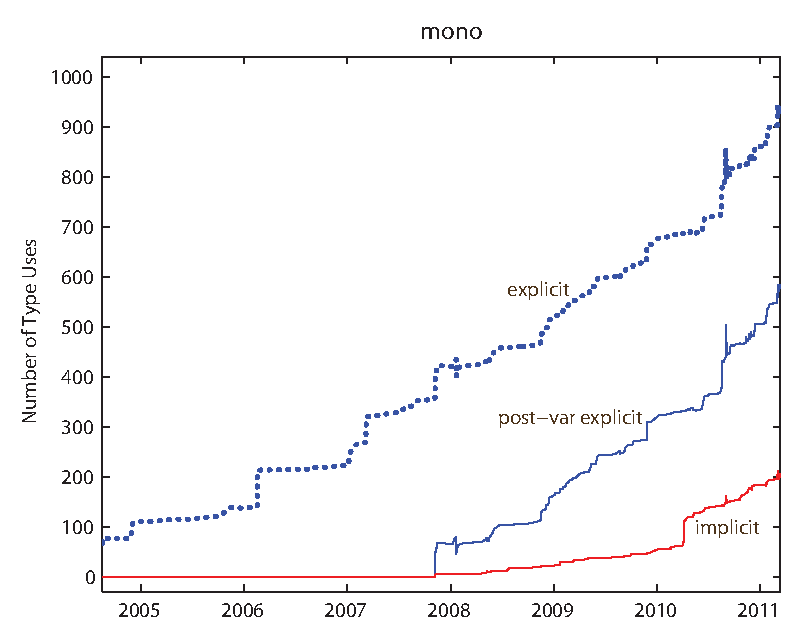
\includegraphics[width=0.7\textwidth]{fig7_mono_implicit2_1117.eps}
\end{center}
\vspace{-15pt}
\setlength{\tabcolsep}{2pt}
\begin{center}
\begin{tabular}{ccc}
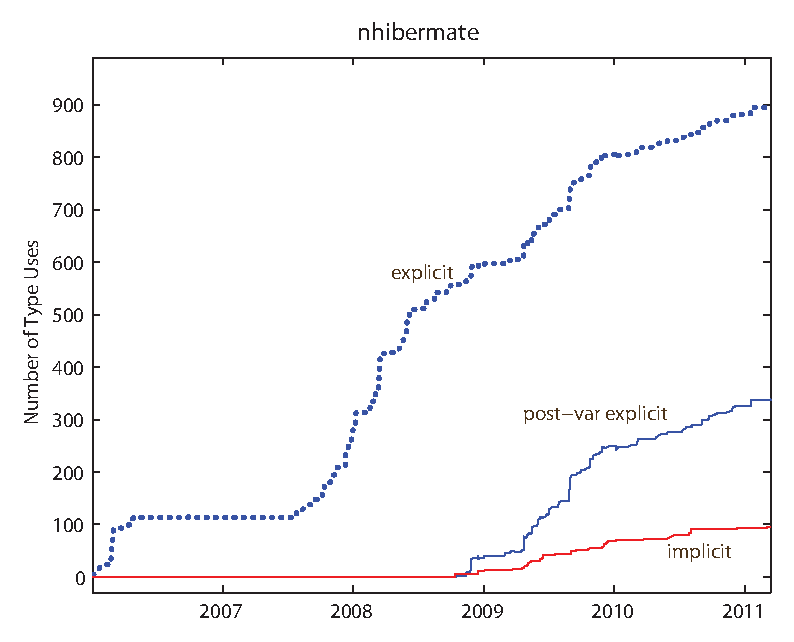
\includegraphics[height=3.5cm]{fig7_nhibernate_implicit2_1117.eps}&
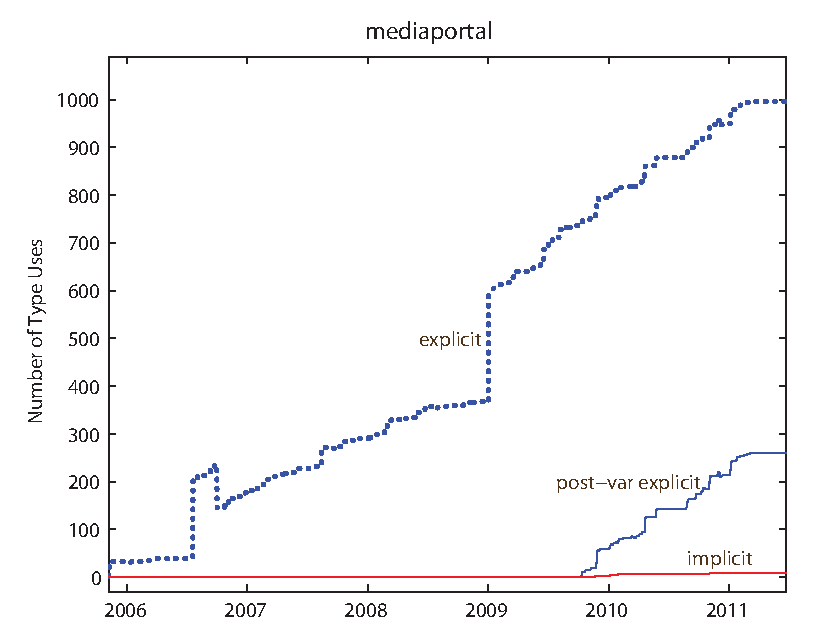
\includegraphics[height=3.5cm]{fig7_mediaportal_implicit2_1117.eps}
\end{tabular}
\end{center}
\vspace{-10pt}
\caption{The usage of implicit and explicit generic declarations over time.}
%\vspace{-10pt}
\label{fig:implicit}
\end{figure*}

%\begin{figure*}[!ht]
%\begin{center}$
%\begin{array}{ccc}
%\includegraphics[width=1.6in]{fig7_mono_transition_implicit.eps} &
%\includegraphics[width=1.6in]{fig7_nhibernate_transition_implicit.eps}&
%\includegraphics[width=1.6in]{fig7_mediaportal_transition_implicit.eps}
%\end{array}$
%\end{center}
%\caption{The number of implicit and explicit generic declarations are added after the first var type over time.
%Explicit generics declarations are used more than implicit ones overall in projects}
%\label{fig:implicit_transition}
%\end{figure*}

%\begin{figure*}[!ht]
%\begin{center}$
%\begin{array}{ccc}
%\includegraphics[width=1.6in]{fig8_mono_var_1117.eps} &
%\includegraphics[width=1.6in]{fig8_nhibernate_var_1117.eps}&
%\includegraphics[width=1.6in]{fig8_mediaportal_var_1117.eps}
%\end{array}$
%\end{center}
%\caption{Contributors' usage of implicit generic declarations over time for the five most active contributors in each project.}
%\label{fig:var_contributors}
%\end{figure*} 

%\begin{figure}[!ht]
%\begin{center}
%\includegraphics[width=2.6in,angle=90]{user-bar-1117-1.eps}
%\caption{Contributors' usage of implicit and explicit generic declarations for most active contributors in each project.}
%\label{fig:var-user-bar}
%\end{center}
%\end{figure}

%[FSE_review]
As explained in Section~\ref{subsection:comparison},
programmers can declare local variables with the \texttt{var} 
keyword instead of using explicitly typed generics.
This may encourage the use of generics because redundancy can be reduced.
At the same time, however, using the \texttt{var} keyword may reduce readability.  
Our research question (RQ6) is whether developers prefer to reduce redundancy
by using the \texttt{var} keyword with generics.
%In addition, the \texttt{var} type declaration does not impact performance at run-time because of compile-time type inference.
To answer this research question, we analyzed the projects looking for 
two different but equivalent programming statements, generic assignments that use
\texttt{var} and assignments that do not use \texttt{var}:
\begin{verbatim}
    var list = new List<String>();
    List<String> list = new List<String>(); 
\end{verbatim}
For simplicity, we limited our analysis to assignments where the variable is declared on
the left hand side of the expression and the right hand side of the expression
is a call to a constructor with one or more generic type arguments.
We then examined how many \texttt{var} types are used over time by each developer in each project.

%Figure \ref{fig:implicit} depicts a gross comparison by showing the growth in explicit types and implicit types over time for the three projects.
Figure~\ref{fig:implicit} shows the numbers of explicit types and implicit types over time.
In the figure, \textbf{explicit} denotes parameterized types defined explicitly and
\textbf{implicit} denotes parameterized types defined with \texttt{var} types.
However, directly comparing these two is not a fair comparison, since 
implicit local variable typing was not available when these projects began.
Therefore, in Figure~\ref{fig:implicit}, \textbf{post-var explicit} denotes that 
the number of explicit parameterized type declarations  
which are added after first introducing the \emph{var} type in a project.
Intuitively, \textbf{post-var explicit} represents a community choice not
to use implicit typing.
Looking at the figures, 
the number of \textbf{post-var explicit}s are always larger than that of \textbf{implicit}.
%The number of \textbf{explicit} is much high than that of \textbf{implicit} in all projects. 
In fact, only 4 out of 19 projects use the \texttt{var} type with local parameterized type variables. 
The percentage of \texttt{var} types for each of \emph{mono}, \emph{nhibernate}, and \emph{mediaportal} 
after their first use of \texttt{var} are 25.7\%, 22.1\%, and 3.3\%, respectively.   
%mono is 203 vs	585, nhibernate is 96 vs 339, mediaportal is 9 vs 260, monodevelop is 82 vs 465
%Specifically, Figure \ref{fig:implicit_transition} represents the number of types added after introducing the \texttt{var} type in a project.
%In these figures, \textbf{explicit} denotes parameterized types defined explicitly,
%\textbf{implicit} denotes parameterized types defined with \texttt{var} types.
%Figure \ref{fig:var-user-bar} %\ref{fig:var_contributors} 
%shows the usage of the generic type declarations for each contributor.
We also found that after using \texttt{var} for the first time,
only 1 out of 30 developers continued to use \texttt{var}
as their preferred way to declare generic local variables.
%out of 30 developers, 27 used explicit more often after their first use of var (2 users are a tie)

%We found that most of the developers used explicit generic type declarations more often than implicit ones    

%Overall, \texttt{var} types for implicit generic declarations are not used actively for all projects.
%We note that only 4 out of 20 projects use implicit generic type declarations: 
%\emph{mono}, \emph{nhibernate}, \emph{mediaportal}, and \emph{monodevelop}. 
%The \emph{mediaportal} project has only 9 \texttt{var} types (\textless 1\%) while it has 1,060 explicit parameterized types. 


%\texttt{var}  types for implicit generics declaration are not used actively for all projects.The \emph{mediaportal} project has only 9 \texttt{var} types (\textless 1\%) while it has 1,060 parameterized types.
%We observed more details for each project. 
%In the \emph{mono} project, the first \texttt{var} type appeared on Nov 8, 2007, the earliest date among all 4 projects.
%The percentage of \textbf{post-var explicit} 
%is 68.0\% while overall percentage of explicit types is 86.5\%.
%The percentage of \textbf{post-var explicit} from the top five contributors is 58.2\% while overall percentage of explicit types is 72.8\%.
%In the \emph{nhibernate} project, the first \texttt{var} type appeared on Oct 11, 2008. 
%The percentage of \textbf{post-var explicit} is relatively high, 81.9\% while it is 91.6\% for overall explicit types.
%In the \emph{monodevelop} project, the first \texttt{var} type appeared on Dec 17, 2008. 
%The percentage of \textbf{post-var explicit} is 88.4\% 
%while the percentage of overall explicit types is 91.5\%. 
%We note that most of developers use explicit generics declarations more often than implicit ones.

Although developers did not appear to use \texttt{var} very often,
we were curious as to whether concision was important to developers at all.
We postulated that if concision is important, developers
would be more likely to use \texttt{var} when creating
a \texttt{Dictionary} than when creating a \texttt{List}
because declaring a \texttt{Dictionary} with generics is more
verbose.
We indeed found that this postulate is true: only 21\% of \texttt{Lists}
were declared with \texttt{var} while 49\% of \texttt{Dictionaries} were. 

Overall, the data and our analysis suggest that 
%(1) implicit generic type declarations with \texttt{var} types are adopted within 1 year in C\# projects.
%The duration of \texttt{var} type adoption is shorter than the generics feature.
(1) the usage of implicit generics declaration is relatively low,
(2) a small number of developers use \texttt{var},
%most of developers prefer explicit ones,
and
(3) developers prefer implicit generic declarations for succinct syntax.
Based on the first two points, 
we conclude that our results suggest that \textbf{developers do not prefer implicit 
type declarations when using generics}.
Although
%the introduction of \emph{var} type could have an positive influence on the usage of generics since
the number of implicit generic declarations is increasing steadily, the \texttt{var} type is not used widely by C\# developers.

%Threats to Validity
%Because we examine \texttt{var} use in only a limited form, 
%there may be other dynamics we are not capturing.  
%For example, developers may be less likely to use implicit declarations for storing the return value of a method call.
%In future work, a deeper semantic analysis could more finely examine these factors.



%[FSE_review]
\subsection{Threats to Validity}
\label{subsection:threats}

Our results have several limitations.
First, our analysis of RQ1 is coarse-grained
in that it looks at general cast and generic trends across
whole codebases.  
With more sophisticated analysis, we may be able to identify individual casts that 
were removed due to using generics 
and compare that with other contexts for removal.   
Second, our analysis of RQ2 only applies to code duplication internal to a project.
One factor that is not accounted for is that some 
generic library classes may be intended for client use.
In those cases, we may be underestimating the amount of code duplication that is reduced. 
Third, our analysis of RQ4 is that 
our heuristic for identifying conversions from raw types to generics
may have counted some changes as migrations when they were not
and vice versa.  However, we evaluated this heuristic in previous
work and found that it was in fact quite precise~\cite{java_generics_ese}.
Fourth, our analysis of RQ5 stems from our static analysis of performance.
There may be other conditions that mask or dwarf the performance gains from value types 
during execution of the program.
In the future, a dynamic analysis of these programs using their own unit tests would 
allow us to more accurately measure what performance gain developers can expect from using generics
with value types. 
Fifth, because we examine \texttt{var} use in only a limited form for RQ6, 
there may be other dynamics we are not capturing.  
For example, developers may be less likely to use implicit declarations for storing the 
return value of a method call.
In future work, a deeper semantic analysis could more closely examine these factors.
%[FSE_review]
Sixth, we included the Mono and MonoDevelop  because they fit our criteria for 
project selection, yet because the developers of these projects are necessarily very familiar
with C\# language features, these two projects are likely not representative of the average C\# project.
Seventh, as we noted earlier, the projects we studied in C\# were substantially smaller than the
Java projects.
This may have some counfounding effects when we compare Java to C\# generics
for the projects we studied.
Finally, the research questions in this paper were formulated and answered 
using quantitative research methods, meaning that we could observe trends,
but only hypothesize why those trends exist. 
To confirm why those trends exist, we must use more qualitative research methods, 
such as interviews with the programmers who created the code.


%%%%%%%%%%%%%%%%%%%%%%%%%%%%%%%%%%%%%%%%%%%%%%%%%%%
%%%%%%%%%%%%%%%%%%%%%%%%%%%%%%%%%%%%%%%%%%%%%%%%%%%
%%%%%%%%%%%%%%%%%%%%%%%%%%%%%%%%%%%%%%%%%%%%%%%%%%%






\section{Discussion}
\label{section:discussion}

\subsection{Design Choice Matters}

In our study, we observed that generics were somewhat, though not statistically significantly, more widely  
used in C\# than in Java (Section~\ref{subsection:projects}),
and also that generics allowed more duplication to be eliminated in C\#
programs than in Java programs (Section~\ref{section:investigating}).
At least in the sense of adoption and duplication elimination, 
why was the introduction of generics in C\# more successful than 
in Java?

One reason for the difference appears to be the way the language
feature was introduced into the two languages.
In Java, language designers allowed existing classes do be ``generified''
without forcing developers of those classes to use parameterized types,
but instead gently encouraging them to do so with compiler warnings.
At the same time, standard Java library maintainers took advantage of
this and generified their collections library, presumably with the hope
that the Java compiler's warnings would encourage end developers to adopt
generics.
In contrast, C\# took a different approach.
While C\# library designers offered generic versions of existing collections,
they also offered a new set of generic collections.
This essentially offered an additional incentive to use generics\textemdash if a developer wanted
to use the new collections, they must learn to use generics.


Our results suggest that this C\# incentive-based approach paid off based on the 
higher adoption rates and higher duplication-elimination, compared with 
Java.
As evidence, as shown in Section~\ref{subsection:feature_breakdown}, 
most generic types used in C\# projects
belong to the \texttt{System.Collections.Generic} namespace,
types that must be used as parameterized types.
This suggests that the newly introduced collections were 
valuable enough that developers were willing to use them,
even if that meant they had to learn a new language feature.
As a result, C\# projects gain the benefits of generics from developers' pains\textemdash ``\emph{No pain, No gain}.''

On the other hand, our results suggest that generics in C\# may
have been a victim of their own success.
Specifically, the rate of end-developer-defined generic types used
with only one type argument was substantially higher than 
in Java; we found about half of these types were
parameterized with only one type 
argument (Section~\ref{subsection:generics_code_duplication}).
One explanation could be that these types were used largely 
in library code, that is, external developers were expected to
parameterize these types with a variety of type arguments,
even if the library's own code did not.
Another explanation is simply over-generalization:
developers anticipated a class would be useful with
a wider variety of type arguments than it actually was.
From our own experience as developers, it is easy
to fall into the trap of being so enamored with the power
of a language feature that you use it in places where it would
do something ``cool,'' even if it is not very useful.

\subsection{Readability Over Concision}

Before the study, we expected that developers would frequently use the
\texttt{var} type to avoid repetition.
Indeed, our finding about using \texttt{var} more commonly with
the two-type argument \texttt{Dictionary<TKey,TValue>} than with
the one-type argument \texttt{List<T>} suggests that
readability is a factor.
However, we were surprised that, overall, developers rarely used 
\texttt{var}, even after they learned how to use it.
We speculate that part of the reason has to do with whether the code
was meant to be read by others.
If the code being written is closed source, is experimental, or is worked on by only one developer,
then the use of \texttt{var} may be a more acceptable practice.
In the projects we studied, which were open-source, mature,
and multi-developer, the use of \texttt{var} may not have been
seen as a collaboration-friendly programming construct.
We plan on investigating the factors that lead to \texttt{var} use
in future work by contacting C\# developers directly.

\subsection{Implications}
Our results have implications for language design and in fact have already begun to
inform language designers.  As an example,
TouchDevelop\footnote{\url{http://www.touchdevelop.com}}, a language designed
to enable easy development for mobile devices on mobile devices,
currently has no support for generics.  
After we discussed our empirical results with the langauge's designers,
they chose not to add support for 
generics in an upcoming release.
They concluded that adding generics would bring too much complexity for 
little gain and most functionality could be provided with special collection libraries based on
our findings (1) that collections of strings (\emph{e.g.} sets, lists,
dictionaries) account for a large majority of generics use and (2) that developers
use standard generic classes much more than they create them.
%, provided insights
%that were able to inform TouchDevelop designers as they considered how and if
%the language should be enhanced.



\section{Conclusion}
\label{section:conclusion}
Throughout the empirical study of C\# generics, 
we investigated the claimed benefits from language designers 
whether the benefits hold in the real open-source projects. 
%In this paper, we conducted an empirical study of 
%C\# generics to analyze how the generics feature is used in C\#. 
We compared the results of C\# generics with those of Java generics.
%Due to the difference such as  \textit{must} or \textit{choice} 
%in generics implementation between C\# and Java, 
The results suggest that the percentage of C\# developers using generics is larger 
than that of Java developers using generics. 
%(2) C\# generics are used widely by most of C\# developers who used parameterized types nevertheless a small number of C\# developers. 
%while Java generics are used by one or two developers than
Specifically, we showed that several benefits of 
the generics feature are manifested more clearly in C\# than in Java.   
%We verified that C\# generics improve performance in a project. 
%C\# generics performance is increased in a project although C\# generics may rarely affect overall performance gain. 
% We also analyzed the usage of implicit generic type declarations, 
% and then found that C\# developers prefer program readability rather than succinct syntax. 
% In our discussion, we claimed that the different implementation of the same language feature may affect the usage of the language feature in programming languages beyond the benefits of the language feature. 
%The distinct characteristics of C\# generics may make different results of the usage of generics compared with Java generics.
%The primary reason we derived from the results is that 
%C\# generics is not a \textquotedblleft choice\textquotedblright \ but a \textquotedblleft must\textquotedblright \ to use new created libraries such as \emph{p-only}.
%In addition, we recognize that implicit generics type declaration is not used widely yet, but used when needed by C\# developers.
%As the contribution we mentioned in introduction, 
%this study verified the claimed benefits from language designers 
%whether the benefits hold in the real open-source projects. 
Based on these results and those for Ada and Java generics, 
we have found that developers may not always reap the benefits of language features
in different implementations.
While our results are interesting, there remain several limitations
to our approach, and further research is necessary to validate whether our 
findings apply more broadly.
%[JOT_review] no change
Nonetheless, we hope that our experimental results can assist
language designers in making evidence-based decisions
when introducing language features, 
which in turn will amplify the benefits of those features in practice.
%\end{document}  % This is where a 'short' article might terminate
\backmatter

\section{Appendix}
\label{section:appendix}

In this Appendix, we show extended figures for all projects. 

\newcommand\figrow[4]{
\begin{tabular}{ccc}
\includegraphics[height=0.25\textwidth]{#1#2}&
\includegraphics[height=0.25\textwidth]{#1#3} &
\includegraphics[height=0.25\textwidth]{#1#4}
\end{tabular}\vspace{-3mm}
}

\newcommand\figrowshort[3]{
\begin{tabular}{ccc}
\includegraphics[height=0.25\textwidth]{#1#2}&
\includegraphics[height=0.25\textwidth]{#1#3}
\end{tabular}\vspace{-3mm}
}

\begin{figure*}[!ht]
\centering
\vspace{-10pt}
\setlength{\tabcolsep}{2pt}
\begin{center}
\figrow{./cast/fig3_}{ankhsvn}{banshee}{beagle}
\figrow{./cast/fig3_}{boo}{Castle}{ccnet}
\figrow{./cast/fig3_}{cuyahoga}{f_spot}{jayrock}
\figrow{./cast/fig3_}{log4net}{lucene_net}{mediaportal}
\figrow{./cast/fig3_}{mono}{mono_tools}{monodevelop}
\figrow{./cast/fig3_}{nasa_exp}{nhibernate}{smuxi}
\figrowshort{./cast/fig3_}{tomboy}{zedgraph}
\end{center}
\vspace{-10pt}
\caption{RQ1 - Cast and parameterized types for all projects (extended Figure 2) }
%\vspace{-10pt}
\label{fig:appendix_rq1}
\end{figure*}
\newpage


\begin{figure*}[!ht]
\centering
\vspace{-15pt}
\setlength{\tabcolsep}{2pt}
\begin{center}
\figrow{./users/fig5_}{ankhsvn}{banshee}{beagle}
\figrow{./users/fig5_}{boo}{Castle}{ccnet}
\figrow{./users/fig5_}{cuyahoga}{f_spot}{jayrock}
\figrow{./users/fig5_}{log4net}{lucene_net}{mediaportal}
\figrow{./users/fig5_}{mono}{mono_tools}{monodevelop}
\figrow{./users/fig5_}{nasa_exp}{nhibernate}{smuxi}
\figrowshort{./users/fig5_}{tomboy}{zedgraph}
\end{center}
\vspace{-10pt}
\caption{RQ3 - Individual developers' introduction and removal of parameterized types for all projects (extended Figure 3) }
%\vspace{-10pt}
\label{fig:appendix_rq3}
\end{figure*}
\newpage


\begin{figure*}[!ht]
\centering
\vspace{-15pt}
\setlength{\tabcolsep}{2pt}
\begin{center}
\figrow{./raw/fig4_}{ankhsvn}{banshee}{beagle}
\figrow{./raw/fig4_}{boo}{Castle}{ccnet}
\figrow{./raw/fig4_}{cuyahoga}{f_spot}{jayrock}
\figrow{./raw/fig4_}{log4net}{lucene_net}{mediaportal_1213}
\figrow{./raw/fig4_}{mono_1213}{mono_tools}{monodevelop}
\figrow{./raw/fig4_}{nasa_exp}{nhibernate_1213}{smuxi}
\figrowshort{./raw/fig4_}{tomboy}{zedgraph}
\end{center}
\vspace{-10pt}
\caption{RQ4 - The number of raw types and parameterized types for all projects (extended Figure 4) }
%\vspace{-10pt}
\label{fig:appendix_rq4}
\end{figure*}
\newpage


%%%%%
%%%%%performance
\begin{figure*}[!ht]
\centering
\vspace{-15pt}
\setlength{\tabcolsep}{2pt}
\begin{center}
\figrow{./performance/fig6_}{ankhsvn1213}{banshee1213}{beagle1213}
\figrow{./performance/fig6_}{boo1213}{Castle1213}{ccnet1213}
\figrow{./performance/fig6_}{cuyahoga1213}{f_spot1213}{jayrock1213}
\figrow{./performance/fig6_}{log4net1213}{lucene_net1213}{mediaportal1213}
\figrow{./performance/fig6_}{mono_1213}{mono_tools1213}{monodevelop1213}
\figrow{./performance/fig6_}{nasa_exp1213}{nhibernate1213}{smuxi1213}
\figrowshort{./performance/fig6_}{tomboy1213}{zedgraph1213}
\end{center}
\vspace{-10pt}
\caption{RQ5 - The percentage of value types used in parameterized types for all projects (extended Figure 5) }
%\vspace{-10pt}
\label{fig:appendix_rq5}
\end{figure*}
\newpage


%\bibliographystyle{abbrv}
%\bibliography{sigproc}

\bibliographystyle{alphaurl}
\bibliography{sigproc}

\abouttheauthors

\begin{acknowledgments}
Thanks to Titus Barik, Xi Ge, Brittany Johnson, Da Young Lee, Jun Bum Lim, Yoonki Song, and Shundan Xiao, all of whom provided valuable feedback.
\end{acknowledgments}
\end{document}
